%--------------------------------------
% Master's Thesis Title Page
% LaTeX Template
% Version 1.0 (23/05/14)
%---------------------------------------

%----------------------------------------------------------------------------------------
%	PACKAGES AND OTHER DOCUMENT CONFIGURATIONS
%----------------------------------------------------------------------------------------

\documentclass[a4paper, 12pt]{report}\dfrac{\right }{•}
\usepackage{helvet}
\usepackage[toc,page]{appendix}
\usepackage[toc,acronym,nomain]{glossaries}
\usepackage{graphicx} % Displaying pictures in the document.
\usepackage[floatrow]{chemstyle} % Displaying figures next to item lists.
\usepackage[hidelinks]{hyperref}
\usepackage{listings} % Adding source code listings.
\usepackage{caption}
\usepackage{algpseudocode}
\usepackage{subcaption}
\usepackage{color}
\usepackage[usenames,dvipsnames]{xcolor}
\usepackage{epstopdf}
\usepackage{gensymb}
\usepackage{mathtools}
\usepackage{courier}
\usepackage{fancyhdr}
 
\fancyhf{}
\rhead{\textbf{\thepage}}
\lhead{\textbf{\rightmark}}

\newglossaryentry{js} 		{ name=JavaScript,	description={A scripting language used in web development}}
\newglossaryentry{cpp} 		{name=C++, description={A object-oriented programming language.}}
\newglossaryentry{sc} 		{name=SystemC, description={A simulation library building on C++}}
\newglossaryentry{sampa}  {name=SAMPA, description={SAMPA ASIC}, plural=SAMPAs}
\newglossaryentry{vhdl}{name=VHDL,  description={A Hardware description language}}
\newglossaryentry{verilog}{name=Verilog, description={A Hardware description language}}
\newglossaryentry{altro}{name=ALTRO, description={ALTRO ASIC}}
\newglossaryentry{zs}{name=Zero Suppression, description={Suppression schema/algorithm}}
\newglossaryentry{pq}{name= Priority Queue, description={Datastructure which sorts elements based on a priority(numerical value)}}
\newglossaryentry{rng}{name= Random Number Generator, description={Computational device designed to generate numbers that lack a pattern}}

\newacronym{lhc}{LHC}{Large Hadron Collider}
\newacronym{cern}{CERN}{European Organization for Nuclear Research}
\newacronym{alice}{ALICE}{A Large Ion Collider Experiment}
\newacronym{tpc}{TPC}{Time Projection Chamber}
\newacronym{tev}{TeV}{Tera Electron Volt}
\newacronym{qcd}{QCD}{Quantum Chromodynamics}
\newacronym{asic}{ASIC}{Application Specific Integrated Circuits}
\newacronym{rcu}{RCU}{Readout Control Unit}
\newacronym{cru}{CRU}{Common Readout Unit}
\newacronym{gbt}{GBTx}{Giga Bit Transceiver}
\newacronym{fec}{FEC}{Front-End Card}
\newacronym{fifo}{FIFO}{First-In-First-Out}
\newacronym{gem}{GEM}{Gas Electron Multiplier}
\newacronym{mwpc}{MWPC}{Multi Wire Proportional Chamber}
\newacronym{fpga}{FPGA}{Field-Programmable Gate Array}
\newacronym{bt}{BT}{Binary Tree}
\newacronym{oop}{OOP}{Object-Oriented Programming}

\makeglossaries
\definecolor{mygreen}{rgb}{0,0.8,0}
\definecolor{mygray}{rgb}{0.5,0.5,0.5}
\definecolor{listinggray}{gray}{0.5}
\definecolor{lbcolor}{rgb}{0.95,0.95,0.95}

\newcommand{\codeword}[1]{\texttt{#1}}

% Solarized colour scheme for listings
\definecolor{variable}{RGB}{43, 145, 175}
\definecolor{keyword}{RGB}{0, 0, 255}
\definecolor{number}{HTML}{0080A0}
\definecolor{string}{RGB}{163, 21, 21}
\definecolor{comment}{RGB}{0, 128, 0}
\definecolor{background}{HTML}{FFFFFF}
\definecolor{function}{RGB}{111, 0, 138}

% Define C++ syntax highlighting colour scheme
\lstset{language=C++,
		backgroundcolor=\color{background},
        basicstyle=\footnotesize\ttfamily,
        numbers=left,
        tabsize=2,
        breaklines=true,
        escapeinside={@}{@},
        numberstyle=\tiny\color{black},
        keywordstyle=\color{keyword},
        stringstyle=\color{string}\ttfamily,
        %identifierstyle=\color{function},
        commentstyle=\color{comment},
       %directivestyle=\color{black},
        frame=single,
        rulecolor=\color{black},
        showstringspaces=false,
        captionpos=b
}
\DeclareCaptionFont{code}{\color{black}}
\DeclareCaptionFormat{listing}{ #1#2#3  }
\captionsetup[lstlisting]{ format=listing, labelfont=code, textfont=code, singlelinecheck=false, margin=0pt, font={bf,footnotesize} }
\floatsetup[table]{capposition=bottom}

\lstnewenvironment{code}[1][]%
{
   \noindent
   \minipage{\linewidth}
   \vspace{0.5\baselineskip}
   \lstset{basicstyle=\ttfamily\footnotesize,frame=single,#1}}
{\endminipage}
%----------------------------------------------------------------------------------------
%	TITLE PAGE
%----------------------------------------------------------------------------------------

\newcommand*{\titlePage}{\begingroup % Create the command for including the title page in the document
\fontfamily{phv}\selectfont
\centering % Center all text

\vspace{200pt}
{\Huge SystemC simulation of the future SAMPA ASIC for use in the ALICE Experiment in Run 3} \\ % Title
\vspace{5pt}

{\Large \textsl{}} % Subtitle or further description
\vspace{50pt}

{\Large{H\r{a}vard Rustad Olsen}}\\ % Author name

\vfill % Whitespace between the author name and the publisher logo

{\Large Master's thesis in Software Engineering at \\
\vspace{10pt}
Department of Computing, Mathematics and Physics, \\
Bergen University College \\
\vspace{10pt}
Department of  Informatics, \\
University of Bergen \\}
\vspace{10pt}
{\large June 2015} % Month and year published


\begin{figure}[h]
		\begin{subfigure}[]{50pt}
			
\includegraphics[width=50pt]{HIB_sort_hovedlogo.eps}
		\end{subfigure}
		\hfill
		\begin{subfigure}[]{50pt}
			
\includegraphics[width=50pt]{uib-logo.eps}
		\end{subfigure}

\end{figure}

\endgroup}

%----------------------------------------------------------------------------------------
%	BLANK DOCUMENT
%----------------------------------------------------------------------------------------

\begin{document}

\pagestyle{empty} % Removes page numbers

\titlePage % This command includes the title page

\newpage


\chapter*{Acknowledgements}
\addcontentsline{toc}{chapter}{Acknowledgments}

\paragraph{•}
Håvard Helstrup, Johan Alme, Dieter, Arild, Christian, (Damian).
\newpage

\phantomsection
\addcontentsline{toc}{chapter}{Contents}
\tableofcontents

\newpage
\phantomsection
\addcontentsline{toc}{chapter}{List of Figures}
\listoffigures

\newpage
\phantomsection
\addcontentsline{toc}{chapter}{List of Tables}
\listoftables

\newpage
\phantomsection
\addcontentsline{toc}{chapter}{Listings}
\lstlistoflistings
\newpage

% Glossary
%\chapter*{Glossary and acronyms}
%\addcontentsline{toc}{chapter}{Glossary and acronyms}
\printglossaries
\newpage
\pagestyle{fancy}
\chapter{Introduction}
\textit{This chapter will cover the motivation, as well as the scope and goal of this report.}

\section{Motivation}
\label{sec:motivation}
\paragraph{•}
The \gls{lhc} at the \gls{cern} is the world's largest particle accelerator, hosting multiple ongoing experiments.
After a run period of more than 3 years, the \gls{lhc} will be shut down from 2018 until 2021\cite{ls2}.
The purpose of this shutdown is to do maintenance on various equipment in the \gls{lhc}, as well as significant upgrades to the different detectors, one of which is the detector for the \gls{alice}.
\gls{alice} consists of multiple sub-detectors, which combined collect an enormous amount of data.
This amount is expected to increase after the shutdown period as the interaction rate of the \gls{lhc} will increase.
Due to the increase in data output, the \gls{alice} collaboration is seeking to upgrade and enhance the detector capabilities.\cite{alice-upgrade}
This includes a partial redesign of the readout electronics, upgrades to multiple sub-detectors and additional hardware upgrades.

\paragraph{•}
The \gls{tpc} is the \gls{alice} detector's main sub-detector for tracking and identifying particles.
A starting design for the new \gls{tpc} readout electronics has been made, and the different components are currently being developed.
As this is still being worked on, many questions about the different components are yet to be answered.
Are the current specifications sufficient to handle the expected increase in output from the detector?
Do they have the necessary bandwidth to be able to send the data with minimal sample loss.
Are the buffer memory enough to handle the traffic.
Is it possible to optimize the current solution in any way?

\paragraph{•}
The previous paragraph provides motivation for us to find a reliable way of determining a sufficient design for the readout electronics, while being both time and cost efficient.
One strategy for solving this problem, which will be further explored in this thesis is creating a simulation of the system.
Doing a simulation requires designing a accurate representation of the readout electronics, and creating a testbench where it is possible to configure and run multiple tests.


\section{Research Question and thesis goal}

\paragraph{•}
Given the motivation and introduction given in section \ref{sec:motivation} the research question for this thesis becomes:

\paragraph{•}
Is it possible to design and implement a simulation which directly represent the readout electronics, and in doing so will it have an optimizing effect?

\paragraph{•}
Further explained, the main tasks of this thesis will be to create a computer model of the main components of the readout electronics, and run multiple simulations on it.
Experimenting with different configurations in order to find bottlenecks, faulty design or areas of improvement.
The experiments should be logged, and the results will be presented in an organized fashion.


\section{Report structure}
Chapter 2 will give the reader the background information to be able to understand the different academic and scientific terms used, as well as some information about the context of the report.
This includes information about \gls{cern}, the \gls{alice} experiment and the physics most relevant to the thesis.
It will discuss the current readout electronics as well as the proposed upgrade.
Chapter 3 is going further into the problem discussed in this report, initial plans on solving the problem, and information about the tools used.
Chapter 4 will talk about the implementation of the simulation, what problems occurred along the way, and the chosen solution.
The chapter will go into the design, as well as code snippets from the implementation.
With the information given in chapter 4, chapter 5 will discuss the results of the different simulation runs, and evaluate the solution.
Chapter 6 will conclude the thesis with some closing words, and work that can be done in the future.


\chapter{Background}
\textit{This chapter will give the reader the background needed to set the rest of the thesis in context.}

\section{CERN}
\paragraph{•}
\gls{cern} is a European research and scientific organization based out of Geneva near the Franco-Swiss border\cite{cern}.
\gls{cern} is a collaboration between 21 countries with a member staff of over 2500, and more than 12000 associates and apprentices.
The organization was founded in 1954 and has since then been the birthplace of many major scientific discoveries.
These are not limited to discoveries in the field of physics, but includes the creation of the World Wide Web\cite{www}.
Currently the biggest project at \gls{cern} is the \gls{lhc} particle accelerator, which serves as the foundation for multiple experiments in the field of particle physics.
% 2 - 3 more sentences about this!

\section{The Large Hadron Collider}
\label{sec:lhc}
\paragraph{•}
Starting up on 10 September 2008, \gls{lhc} is the latest construct added to \gls{cern}'s particle accelerator complex\cite{lhc}.
It consist of a 27 kilometer underground ring of superconducting magnets which boost the energy of the particles travelling inside the collider.
The collider contains two adjacent parallel high-energy particle beams.
These beams consist of protons extracted from hydrogen atoms by stripping them of electrons.
Along the collider there are four intersection points where collisions occur.
Each point corresponds to the location of a particle detector - ATLAS, \gls{alice}, CMS and LHCb.
The particle detectors are each built and operated by large collaborations, with thousands of scientists from different institutes around the world.
The beams travel at close to the speed of light and are guided by magnetic fields, which are created and maintained by superconducting electromagnets.
Superconducting meaning that it is in a state where it can most efficiently conduct electricity, without resistance or energy loss.
Achieving this state requires cooling the magnets to -271.3\degree~C , which is done by the distribution of liquid helium.
The layout of the \gls{lhc} ring as well as its four collision points can be seen in \ref{fig:lhc}.

\begin{figure}[h!]
  \centering
    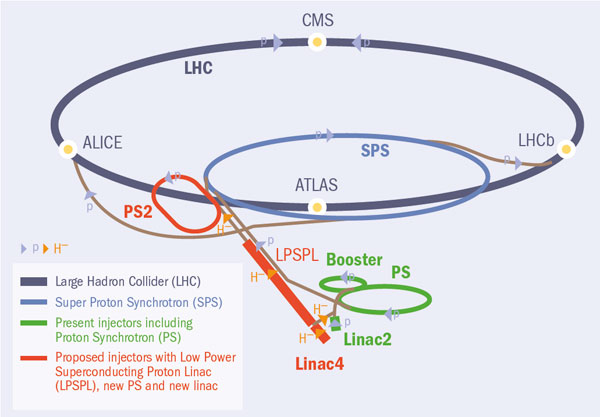
\includegraphics[width=0.7\textwidth]{images/lhc-ring.jpg}
     \caption[The Large Hadron Collider]{The Large Hadron Collider \cite{lhc-ring-image}}
    \label{fig:lhc}
\end{figure}

\paragraph{•}
The beams travelling inside the \gls{lhc} reach an energy-peak of 7 \gls{tev}, which means that on impact with each other the collision reach an energy of 14 \gls{tev}\cite{lhc-pdf}.
During a normal run of the collider there will be about 600 million particle collisions per second during a period of 10 hours.
This leads to a huge amount of data for each of the detectors to read out.
\gls{alice} is the detector which produce the most data per collision, with a design value of about 1.25 GB/s written to permanent storage.
The high amount of data per collision is produced primarily by the \gls{tpc} sub-detector, which records a high number of points per track, and has a low momentum threshold. Detectors like ATLAS and CMS  are designed with a higher momentum threshold, but can cope with significantly higher collision rates than ALICE.
ALICE is designed for the study of heavy ion reactions, where particle correlations at low momentum is an important measure.
The number of tracks correlating with momentum is exponentially declining.
This means that a lot of tracks which do not get registered in ATLAS, produce data in \gls{alice}.

\section{ALICE}
\subsection{Introduction}

\paragraph{•}
\gls{alice} is designed as a heavy-ion detector, which means it studies collisions between heavy nuclei of high energy\cite{alice-home}.
The experiments are run with two different particle collision systems, lead-lead(Pb-Pb) and lead-proton(Pb-p)
Both systems produce an extreme amount of temperature and density.
They produce different, but equally interesting results.
Pb-Pb collisions create Hot Nuclear Matter, while Pb-p create Cold Nuclear Matter.
The explanations for these types of matter is beyond the scope of this thesis and will not be discussed further.
The high temperature and density is necessary to produce a phase of matter called quark-gluon plasma.

\subsection{Quark-gluon plasma}
\paragraph{•}
Shortly after the Big Bang, the universe was filled with an extremely hot cluster of all kinds of different particles moving around at near the speed of light\cite{alice-physics}.
Most of these particles were quarks, fundamental building blocks for matter, and gluons which ties quarks together in order to form heavier particles.
Normally quarks and gluons are very strictly tied together, but in the conditions of extreme temperature and density as in the time shortly after the Big Bang, they are allowed to move freely in an extended volume called quark-gluon plasma.
The existence of quark-gluon plasma and its properties is one of the key issues in \gls{qcd}.
The \gls{alice} collaboration studies this, observing how it behaves.

\subsection{The detector setup}
\paragraph{•}
The detector weight is about 10,000 ton, it is 26 m long, 16 m wide, and 16 m high\cite{alice-about}.
It consists of 18 sub-detectors, each with its own set of tasks regarding tracking and identifying particles.
This large number of sub-detectors are needed in order to get the full picture of the complex system which is being studied(i.e different types of particles and the correlations between them).
Most of the detector is embedded in a magnetic field, created by a large solenoid magnet, which makes particles formed in collision bend according to their charge, and behave differently relative to their momentum. High momentum equals near straight lines while low momentum makes the particles move in spiral-like tracks.
During lead to lead collisions the collision rate peaks at 8 kHz(Where Hz is defined as number of events per second).
The number of recorded events is smaller in practice because the \gls{alice} detector uses a triggered readout, which only triggers on head-on(central) collisions.
The maximum readout rate of the current \gls{alice} detector is 500 Hz, which is more than enough to track central collisions.
\ref{fig:alice} shows a cross section of the detector as it is today with the red solenoid magnet, and all sub-detectors labeled.

\begin{figure}[h!]
  \centering
    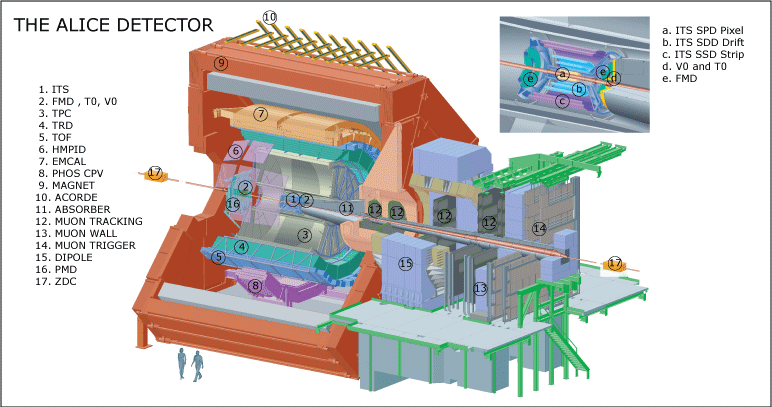
\includegraphics[width=1.0\textwidth]{images/alice-detector.png}
     \caption[The ALICE detector]{The ALICE detector \cite{alice-image}}
    \label{fig:alice}
\end{figure}

\section{The TPC detector}
\subsection{Intro}
\paragraph{•}
One of the most important sub-detectors, and the one that is relevant for this thesis is the \gls{tpc} detector.
Located at the center of the \gls{alice} detector it is among the first entry points when gathering data from a particle collision.
It is a 88\(m^3\) cylinder filled with gas.
The gas works as a detection medium, which means that charged particles from a collision crossing will ionize the gas atoms, freeing electrons that move towards the end plates of the detector.
The readout is done by specially designed readout chambers, which are capable of handling the high amount of data produced in heavy-ion collisions.

\subsection{Readout electronics} %Should this be a chapter of itself?
\paragraph{•}
Signals from the readout chambers are passed along to the front-end readout electronics, which today consist of 4356 \gls{altro} \gls{asic} chips\cite{altro}.
\gls{asic} is the term used for specially customized chips, rather than chips with a more general-purpose use\cite{asic}.
The \gls{altro} chip is made up of 16 asynchronous channels that digitize, process and compress the analogue signals from the readout chambers.
It operates on a so called triggered readout mode.
In short when \gls{altro} receives the first trigger, it stores the following data stream into memory, holding on to it until it is ready to pass on the data.
The front-end electronics are able to readout data at a speed of up to 300 MB/s.
\paragraph{•}
The \gls{fec} sends the digitized signals further down the readout chain to the \gls{rcu}, where it is further processed and shipped to  and stored in the online systems.
The schematics is shown in \ref{fig:altro}.

\begin{figure}[h!]
  \centering
    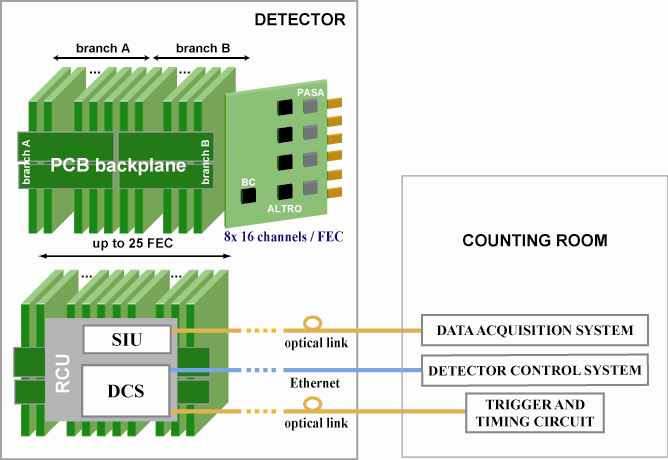
\includegraphics[width=0.75\textwidth]{images/altro.png}
     \caption[Readout schematics for the current TPC detector]{Readout schematics for the current TPC detector \cite{tdr-016}}
    \label{fig:altro}
\end{figure}

\section{Long Shutdown 2}
\paragraph{•}
As mentioned in \ref{sec:motivation} the \gls{lhc} ring will be shut down for about 3 years, starting 2018.
During that time the \gls{alice} detector will undergo an extensive upgrade.
The upgrade strategy for \gls{alice} is based on the expected increase in collision rate to 50 kHz, and will now track every collision.
Essentially this comes down to a increase by a factor of 100, compared to what is achievable today.

\paragraph{•} 
To be able to handle the increase in collision rate the \gls{tpc} will receive upgrades to both its readout chambers, and front-end readout electronics.
The current \gls{mwpc} based read-out chambers will be replaced by \gls{gem} detectors, which has a much higher readout rate capability.
Signals will be passed from the new readout chambers to the \gls{fec} via a readout pad structure similar to the one presently used.
There are multiple pad structures depending on its location on the detector, but the difference in structure is not relevant for this thesis.
What is relevant however is that more data is expected from low pad numbers, an example of a pad structure is shown in \ref{fig:pad-struct}.

\begin{figure}[h!]
	\centering
		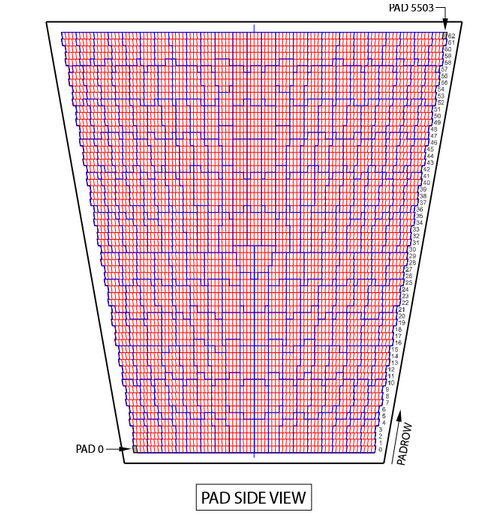
\includegraphics[width=0.75\textwidth]{images/pad-structure.png}
		\caption[Pad structure of an Inner Readout Chamber(IROC)]{Pad structure of an Inner Readout Chamber(IROC)\cite{pad-structure}}
		\label{fig:pad-struct}
\end{figure}

\paragraph{}
The entry point in the \gls{fec} is the new custom-made \gls{asic}, the \gls{sampa}, which will replace the \gls{altro} chip\cite{tdr-015}.
The \gls{sampa} chip is capable of processing signals asynchronously in 32 individual channels, each channel is directly connected to a single pad.
They are further on digitized and concurrently transferred to the \gls{gbt}, which enhances the signal strength and transmits them via multiple optical fiber links to the \gls{cru}.
The \gls{cru} can be thought of as the new \gls{rcu} and serves as an interface to the online systems.
The data flow from the detector, and a working schematics can be seen in \ref{fig:fec}.
Chapter~\ref{cha:4} will go into more detail about the readout electronics in the context of our simulation.

\begin{figure}[h!]
	\centering
		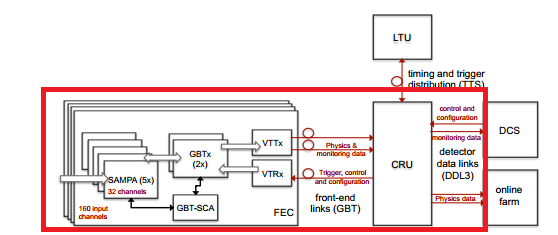
\includegraphics[width=0.75\textwidth]{images/fec.png}
		\caption[Schematics of the readout electronics]{Schematics of the readout electronics \cite{tdr-016}}
		\label{fig:fec}
\end{figure}

\chapter{Simulations}
\label{cha:3}
\textit{SystemC, Starting design of the simulation, plans for implementation and test runs}

\section{Simulation Theory}

\subsection{Theory}
\paragraph{•}
A simulation can be seen as the imitation of a real-world system and its operations over time.
This requires a model representation of the system which is accurate enough to conduct experiments on, which produce real-like results.
The model should include key characteristics, specifications and functions of the selected system, but in a simplified fashion.
A simulation model can take many forms as it can be used in different contexts ranging from physical object such as electrical circuits, bridges, and even entire cities to abstract systems like a mathematical equation or a scientific experiment\cite{simulations}.

\paragraph{•}
As the model represent the system itself, the simulation represents its operations over a set period of time.
The simulation is normally conducted in a controlled environment that makes it possible to observe, monitor and log results.
To achieve efficient experiments using a simulation, it should be easy to change its parameters with respect to what is being tested.

\paragraph{•}
There are many benefits of simulating a system instead of creating and test the real thing.
A simulation will in most cases be very time efficient, you can conduct the same kinds of experiments on the system in a much shorter time compared to the real thing.
This means that more information about the systems behavior and its limitations can be gathered in less time, which in turn can result in a better final product.
Creating the real-world system can often be very expensive, which may limit the amount of prototypes or test-products that are possible to create.
Therefore using results of a simulation to fine tune the specifications before starting to produce prototypes will cut unnecessary development costs by a significant margin.

\paragraph{•}
Taking the upgrade of the readout electronics for the \gls{alice} detector as an example to further address this point one can see the usefulness of not having to create multiple custom hardware components, all with different purposed specification.
In regards to the readout electronics, another important point is that the proposed designs might already function properly, but there is always room for improvement.
Finding out that the design doesn't need as much memory, or less optic fiber cables can impact the overall production costs.
One way to efficiently and accurately simulate hardware components is by creating a virtual computer simulation.

\subsection{Computer Simulations}
\paragraph{•}
Using computers to do simulations becomes more and more useful because of their incredible computational power, and ability to produce fast results.
This is important as simulations often become quite complex, both in regards to computational complexity and level of difficulty to understand and further work with.
Therefore it can be wise to use existing tools to help make the process easier.
There is an array of different tools that can be used to various kinds of simulations.
They vary from complete frameworks, with graphical user interfaces to tools which help programmers write there own simulation programs.
The later requires of course the most work, but will most often end with the better results as you can tailor your simulation on a lower level than with a complete framework.
A programming tool that is made for creating simulations is the \gls{sc} library, which will be discussed in the following section.

\section{SystemC}
\textit{Explain how SystemC works, what benefits and downsides}

\subsection{Background}
\paragraph{•}
\gls{sc} is a system design library based on \gls{cpp}\cite{systemc}.
It provides an interface to easily create a software model that represents a hardware architecture, and together with standard \gls{cpp} development tools it is possible to quickly build a full scale simulation.
Following the standards of \gls{cpp}, \gls{sc} is built to be easy to understand for both software and hardware developers, resulting in clearer cooperation between them while developing the hardware design.
The \gls{sc} library provides an object-oriented approach to model design, where a single \gls{cpp} class represents a model.
This makes it easy to separate concerns between the different models in your simulation.

\paragraph{•}
When simulating a hardware system there is a couple of key points to be aware of, firstly you need to be able to handle hardware timing, clock cycles, and synchronisation.
One of the benefits of \gls{sc} is that it takes care of all of this, again taking advantage of the object-oriented nature of \gls{cpp} to extend its capabilities through \codeword{classes}.
Here are some of the other features \gls{sc} provides, with emphasis on the ones needed to understand code snippets shown in this thesis.

\paragraph{•}
\begin{itemize}
\item \textbf{Modules}
	\begin{itemize}
		\item Container \codeword{class} representing a hardware model.
	\end{itemize}
\item \textbf{Processes}
	\begin{itemize}
		\item In short, processes are methods inside a module which describe the module functionality.
	\end{itemize}
\item \textbf{Ports}
	\begin{itemize}
		\item Ports represent the input and output points of a module, they can be connected to other modules through Channels.
		When you declare a port in a simulation, it is required to specify if the port is an input, output or bidirectional port.
		This is done by specifying a channel interface for the port.
		Example of a port using a input \gls{fifo} interface: \begin{verbatim}sc_port<sc_fifo_in_if>\end{verbatim}.
	\end{itemize}
\item \textbf{Channels}
	\begin{itemize}
		\item Channels are the wires connecting two Ports.
		\gls{sc} comes with three predefined channels: \gls{fifo}, mutex, and semaphore.
		It is possible to configure custom channels, but in most cases it is not necessary.
	\end{itemize}
\item \textbf{Signals}
	\begin{itemize}
		\item Signals represent data sent between modules via ports.
		They can be arbitrary data types like \codeword{bool} or \codeword{int}, but also user defined types.
	\end{itemize}
\item Rich set of data types
	\begin{itemize}
		\item \gls{sc} supports all data types defined in \gls{cpp} as well as multiple custom types.
	\end{itemize}
\item Clocks
	\begin{itemize}
		\item \gls{sc} comes with clocks, which can be seen as timekeepers of the system during a simulation.
	\end{itemize}
\end{itemize}

\newpage
\subsection{Small example}

\paragraph{•}
To get a basic understanding of how a \gls{sc} simulation looks like, it is useful to see it in action.
The following \ref{fig:sc-ex} and Listings~\ref{lst:prod-ex}-\ref{lst:main-ex} make up a very trivial example with only 2 modules; a \codeword{Producer} and a \codeword{Consumer}.
The \codeword{Producer} will increase a counter every clock cycle, and send a \codeword{bool} value based if the count is an even number, and send this value to the \codeword{Consumer}, which registers how many times the \codeword{Producer} counted an even number.
The example uses a \gls{fifo} channel, connected between an output port on the \codeword{Producer}, and an input port on the \codeword{Consumer}.

\begin{figure}[h!]
  \centering
    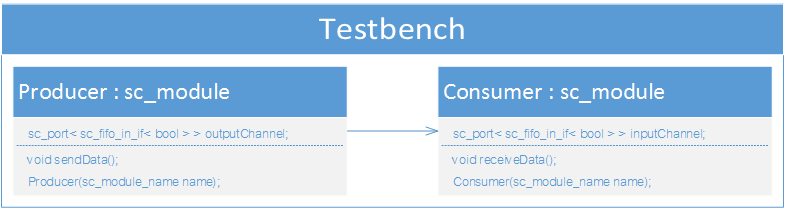
\includegraphics[width=1.0\textwidth]{images/sc-example.png}
     \caption{Basic SystemC example}
    \label{fig:sc-ex}
\end{figure}

\noindent
\begin{minipage}{\linewidth}
\lstinputlisting[caption=Producer module.,label=lst:prod-ex]{codelistings/producer.cpp}
\end{minipage}
\begin{minipage}{\linewidth}
\lstinputlisting[caption=Consumer module.,label=lst:cons-ex]{codelistings/consumer.cpp}
\end{minipage}
\begin{minipage}{\linewidth}
\lstinputlisting[caption=Simulation test-bench.,label=lst:main-ex]{codelistings/main.cpp}
\end{minipage}

\paragraph{}
\gls{sc} can be used to create very low level hardware descriptions and models, and can interface directly with hardware description languages like \gls{vhdl} and \gls{verilog}.
This is one way to create a simulation, and the models will be very accurately represented by doing so.
The other way is to have a high level of abstraction, leaving out the unimportant details and focus solely on the expected problem areas.
There are benefits and drawbacks for both ways, but sticking to a high abstraction level can in complex cases make it a lot easier to work with the model design and allows you to focus on the important parts.

\chapter{Problem Description}
\textit{Explain the model, introduce the problem}
\label{cha:4}

\paragraph{}
The previous chapters have briefly introduced the problems of this thesis, relevant background information and looked at tools and the method of solving them.
Essentially it boils down to creating a model based on the schematic of the \gls{tpc} readout electronics, run multiple simulations, testing different parameters for the involved components.
Until now there has only been an introduction level description of the different components that is being included in the simulation model.
This chapter will go deeper into them, giving detailed information about their design parameters, and how the \gls{alice} experiment data is handled by them.
Not going too far into the task of implementing this in a \gls{sc} environment, but focus on the different problem areas, what is required in order to solve them and what goals to achieve.

\section{Model Design}
\textit{Different design patterns, and plans for the electronics}
\paragraph{}
The hardware design which is being simulated is already briefly shown in \ref{fig:fec}.
The proposed schematic shown there consists of 12 \gls{fec} cards for every \gls{cru}.
Each \gls{fec} consists of 5 \gls{sampa} and 2 \gls{gbt} \glspl{asic}, with the \gls{cru} being connected to them via 24 optical links.
Out of the 3 main chips, the \gls{sampa} and the \gls{cru} are the most interesting as they are still being developed and testing them can give a lot of valuable feedback.
The \gls{gbt} is a completed component, so even though it is part of readout electronic being simulated, it will only be a very shallow abstraction of it.
This means that it will remain as an empty module whose objective will be to just pass along received data to the correct output links.
One important note about the \gls{gbt} input and output links.
Each \gls{gbt} has 10 input e-links, each with a transfer rate of 320 Mbit/s, giving an effective input speed of 3.2 Gbit/s per \gls{gbt}.
The output is 1 optical fiber link with a speed of 3.2 Gbit/s, giving the \gls{gbt} the same input and output speed.
This is the reason letting data flow directly through the \gls{gbt} in the simulation is possible.
The next sections will go into details about the more important components.

\subsection{SAMPA}
\label{subsec:sampa}
\paragraph{}
The \gls{sampa} \gls{asic} is based on the work from its predecessor, the \gls{altro}.
Just like the \gls{altro} it will be the first step for signals being tracked in the \gls{tpc} detector.
The signals will be processed, compressed, digitized, and temporarily stored in the \glspl{sampa} memory before they are passed along.
The \gls{sampa} has 32 integrated channels, which separately and asynchronously process the analog signals coming from the detector\cite{tdr-016}.
Each channel has a readout speed of 10 bit on a 10 MHz clock, which combined results in 3.2 Gbit/s.
The channels also have their own \gls{fifo} buffer memory where signals coming in are stored as they wait to be sent along.
The most efficient size for these buffers are one of the things the simulations will hopefully provide.
The output links for the \gls{sampa} chip consists of 4 e-links connecting them to the \gls{gbt}.
Each e-link has as said in the previous section a speed of 320 Mbit/s, which sums up to 1.28 Gbit/s\cite{tdr-015}.
The e-links are connected to 4 readout buffers on the \gls{sampa} that reads from the channel buffers and transports the data to the e-links.
The readout buffers reads from 8 channels each.
Since each \gls{sampa} and \gls{gbt} has a specific number of output and input links, there are only certain setups which are desirable.
This is why the proposed schematic uses 5 \gls{sampa} and 2 \gls{gbt} chips for each \gls{fec}.
That setup gives exactly 20 output links from the \gls{sampa} chips, and 20 input links on the \gls{gbt} chips.

\paragraph{}
As the \gls{altro}, the \gls{sampa} can be run in triggered readout mode, but in addition it can be run continuously.
Being able to read out continuously is a necessary upgrade to handle the increased data load coming from the detector.
During continuous mode the data acquisition is uninterruptable, meaning that there is no pause between reading two consecutive events from the detector.
The difference it makes compared to triggered mode can be seen in \ref{fig:cont-vs-trig}.
Every event, from now on referred to as time frames, is 1024 clock cycles long, and all 32 channels of the \gls{sampa} use the same time frame.
This means that every 1024 clock cycle a 1024 long time window is initiated for all 32 channels, meaning they can readout 10 bit data samples 1024 times during this window.
A synchronization input allows multiple \gls{sampa} \gls{asic}s to align their time frames with respect to each others.\cite{tdr-015}

\begin{figure}[t!]
	\centering
		\begin{subfigure}[]{0.9\textwidth}
			\label{fig:cont}
			\includegraphics[width=\textwidth]{images/cont-mode.png}
		\end{subfigure}
		\begin{subfigure}[]{0.9\textwidth}
			\label{fig:trig}
			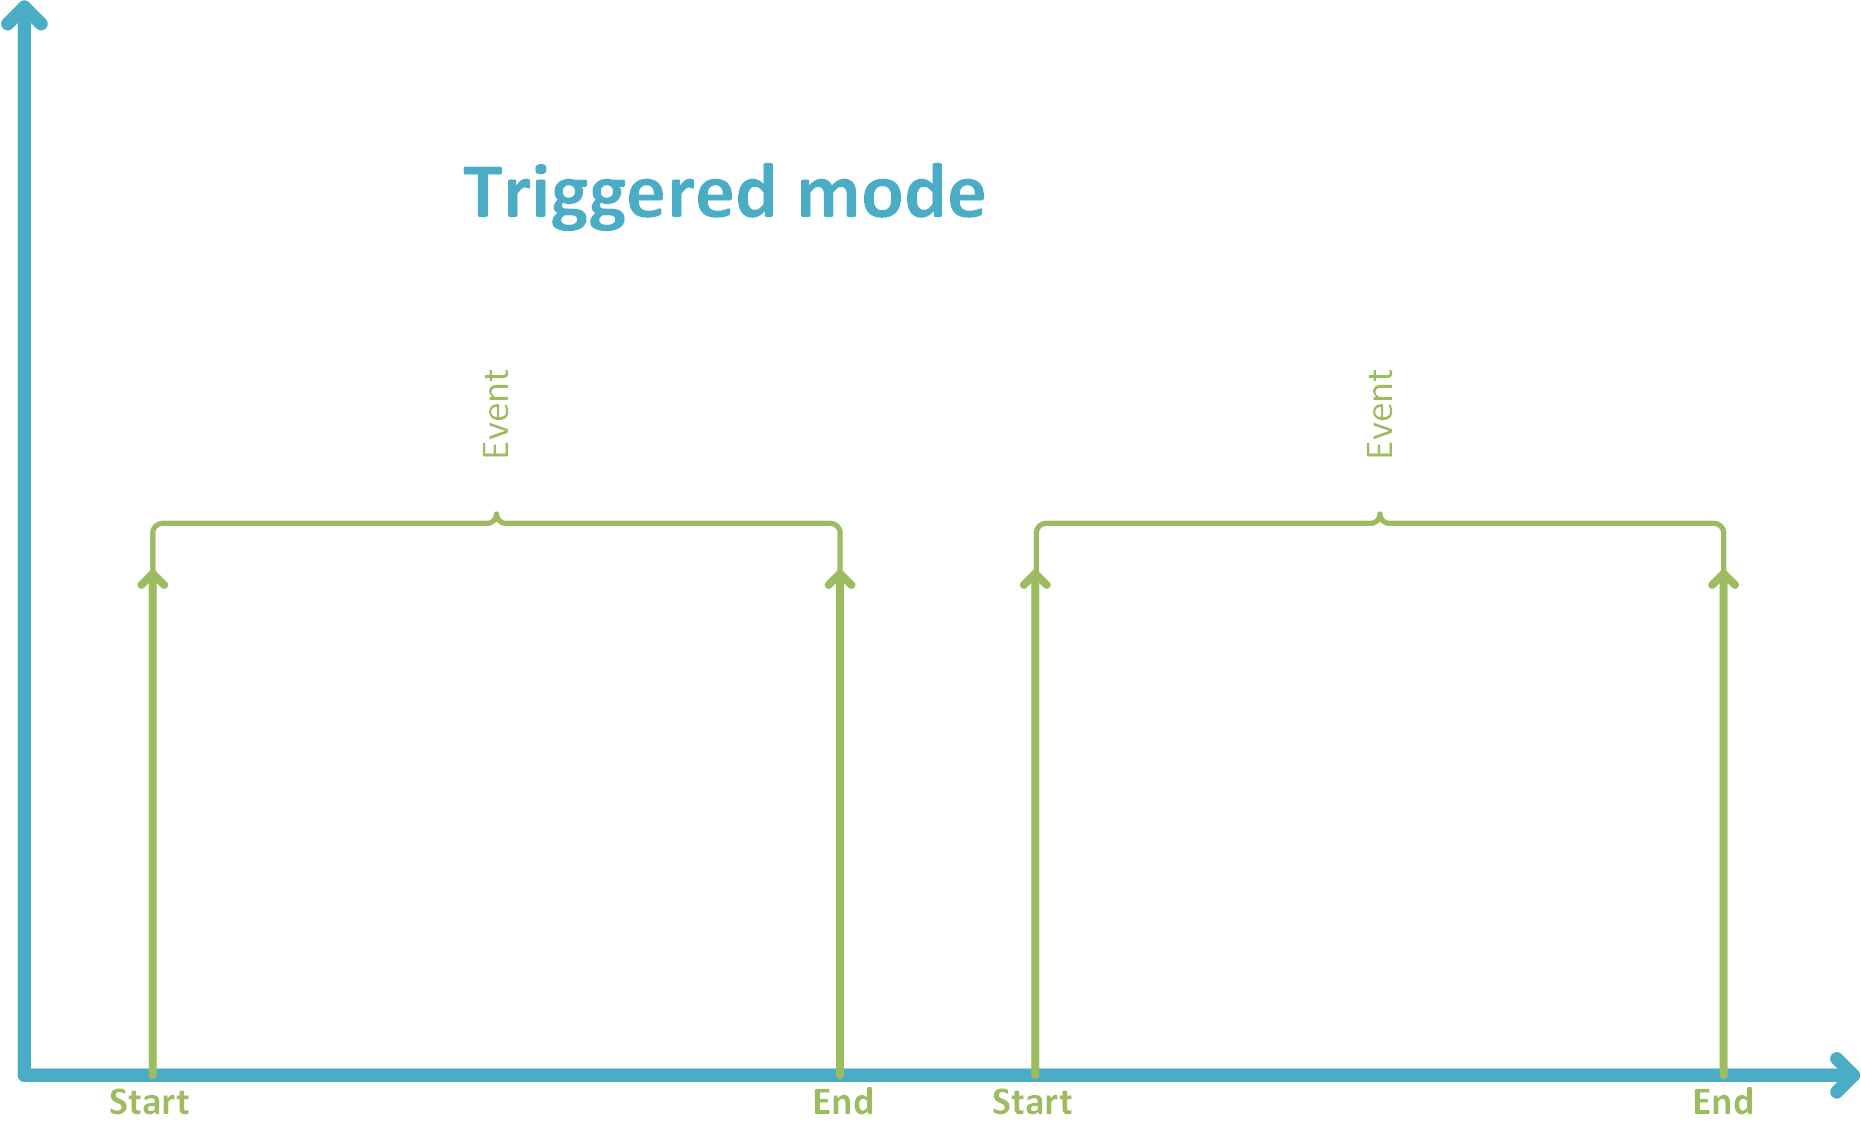
\includegraphics[width=\textwidth]{images/triggered-mode.png}
		\end{subfigure}
	\caption{Continuous vs Triggered mode}
	\label{fig:cont-vs-trig}
\end{figure}

\paragraph{}
The \gls{sampa} creates data packets from the data assembled from each time frame.
Consisting of a header of fixed size 50 bit, followed by a list of 10 bit samples, created from a single time frame.
Even though a time frame consists of 1024 clock cycles, in practice a maximum of 1022 samples are received each time.
This is due to the fact that 2 * 10 bit words are required to represent cluster size (size of consecutive samples) and a timestamp.
The headers are stored in their own \gls{fifo} buffers, separate for each channel, much like the sample buffers.
\ref{fig:packet} shows the structure and format of the packets.

\begin{figure}[h!]
	\centering
		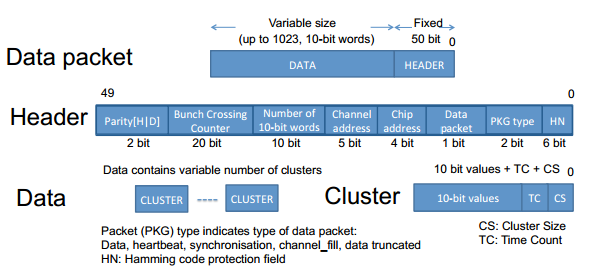
\includegraphics[width=1.0\textwidth]{images/packet.png}
		\caption[Data packet format]{Data packet format \cite{tdr-015}}
		\label{fig:packet}
\end{figure}

\paragraph{}
The header consists of information regarding the data, such as address for the channel and chip, number of data words in the time frame and packet type.
The packet type is used as a marker to see if anything out of the ordinary has happened to the data.
This can be if there is no samples in the time frame, causing the packet type to just become a channel fill packet.
It can indicate if the stream of data was cut short because the \gls{fifo} buffer was full, causing buffer overflow.
In case of buffer overflow all data for the particular time frame are discarded and the empty packet is sent with type overflow.
Overflow can cause a lot of data to get discarded if the \gls{sampa} can't empty the buffers fast enough, this can happen if the buffers don't have enough space.
As the input rate is 3.2 Gbit/s and the readout speed is 1.28 Gbit/s, the \gls{sampa} can receive up to 2.5 times more data per second than it can pass along.
This is why the \gls{fifo} buffers are necessary, and finding a size which is sufficient, without giving overflow is crucial.

\paragraph{}
There have been done some calculations on how much data will actually be received from the detector at any given time.
It is estimated that on average over all channels for every \gls{sampa} there is around 30\% occupancy.
This means that on a global average there is 30\% data in every given time frame.
Some channels may be full while others are empty, and some may have 40\%, but on average there is 30\%, which means 306 samples out of 1022 for every time frame.
Taking this into account when calculating the input speed of the \gls{sampa} gives 960 Mbit/s which the design should be able to handle without any buffer overflow.
Even though there is an estimated average occupancy there can still be some channels which time frame after time frame gets a lot more then that, so how much can the design handle?
This is some of the question the simulation will give answers to.

\subsection{CRU}
The \gls{cru} serves as an interface between electronics directly on the detector and the online computing systems.
It is based on high performance \gls{fpga} processors, with optical fiber used as input and output \cite{tdr-015}. 
The \gls{cru} is somewhat out of the scope of the thesis, and will be regarded in the same fashion as the \gls{gbt}.
How the \gls{cru} is implemented in our design model has no effect on the tests which are going to be performed on the \gls{sampa} and its channels.
It is discussed in the thesis work of Damian K Wejnerowski, who is simulating the \gls{cru} and inspecting it in great detail.

\section{Signal processing in the SAMPA}
\paragraph{}
The \gls{sampa} chips will receive and process a huge amount of data, both relevant signals and background noise.
In section~\ref{subsec:sampa} we talked about occupancy and amount of samples in each time frame.
The estimated amount of 30\% refers to relevant samples, removing or compressing the background noise.
Seeing as it will always be some interference in the background, there will always come samples with data, and gathering all will be a waste of time and space that could be used on the actual collision data in the detector.
\ref{fig:signal} shows 2 actual events collected from the 2 different \gls{altro} channels, the events will look similar after the upgrade and we can use this as a starting point.
The x-axis expresses the current time bin within a time frame from 0 to 1021.
Here one can see that every sample in the time frame has some value most with 48-52, as well as certain peaks here and there.
Those peaks or pulses are what is interesting, everything else is considered noise and should be removed.
In order for any compression schema or method of reducing noise to be valid it needs to have a compression factor above 2.5 for the average amount of data being processed.
The compression factor will be the number of bits in a time frame before compressing compared to after. \codeword{factor = (bits before compression / bits after)}.
There are a number of ways to reduce the amount of noise, and/or compress the data to a manageable size.
What has been used with the current setup and is also discussed to use in in the upgraded setup is \gls{zs}.

\begin{figure}[t]
	\centering
		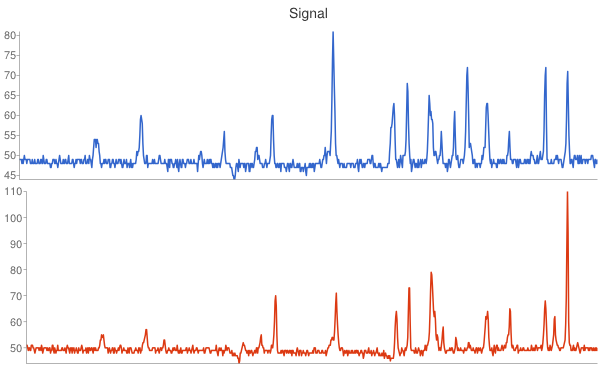
\includegraphics[width=1.0\textwidth]{images/signal.png}
		\caption{Two signals from RUN 1.}
		\label{fig:signal}
\end{figure}

\subsection{Zero suppression} 
\label{subsec:zs}

\paragraph{}
\gls{zs} is the process of removing insignificant values below a set threshold or baseline\cite{zerosuppression}.
Applying this in order to remove the background noise without discarding any important samples, a baseline for the \gls{zs} must be established.
The problem with this is that the baseline may shift, in the case of our 2 example time frames the first one has a visibly lower baseline by 1 or 2.
In the upgrade plans described in \cite{tdr-015}, it is specified how the signal processing will take place.
It works by looking at consecutive signals with value over the set threshold, confirming that the peak is indeed a real pulse.
The term real pulse refers to a sequence of signals over the threshold with more than one signal, standalone values over the threshold will be discarded.
The difference is displayed in \ref{fig:minseq}.

\begin{figure}[h!]
	\centering
		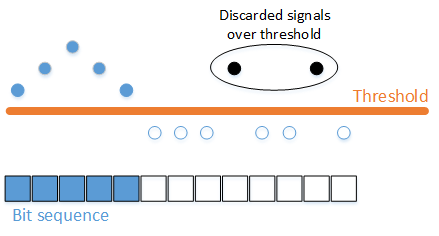
\includegraphics[width=0.75\textwidth]{images/minseq.png}
		\caption{Difference between a valid and invalid signal sequence.}
		\label{fig:minseq}
\end{figure}

\paragraph{•}
Because of the fact that \gls{zs} removes signals from various places in a time frame, the data looses its temporal positioning.
Therefore every real pulse must be tagged with a time stamp and a word representing the number of words in the pulse.
Since for every pulse we add two words, if two consecutive pulses are closer than three words they are merged and counted as one (\ref{fig:merge}).

\begin{figure}[h!]
	\centering
		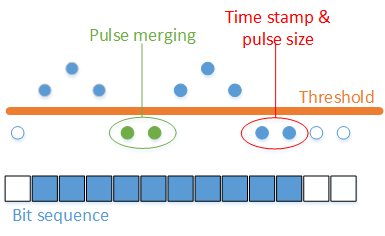
\includegraphics[width=0.75\textwidth]{images/merge.png}
		\caption{Merging of two pulses and the storing of extra pulse information.}
		\label{fig:merge}
\end{figure}

\paragraph{}
In some later discussion regarding the upgrade there has been questions if the described method is insufficient.
The theory behind the discussion is that the baseline will shift too much to be able to do efficient \gls{zs} without loosing important samples in the process.
Another argument against \gls{zs} is that with time frames with larger occupancies (40\%++) the compression factor is drastically reduced and will not be good enough.
This is because time frames with higher occupancy will have more signal pulses, and pulses will be closer together, meaning that more pulses will be merged rather than discarded. 
This encourage finding another way of processing the signals.
One proposed method is to use Huffman coding on the signal values.

\subsection{Huffman Coding} %Only real data
\paragraph{}
Huffman is a method used to achieve data compression\cite{huffman}.
It works by assigning binary codes to symbols in order to reduce the number of bits used to encode the symbol.
By looking at the frequency of appearance for every symbol used one can produce a frequency table sorted by most frequent.
One thing to note is that since the binary codes are of variable length, they may not all be uniquely decipherable.
For instance, if the codewords looks like the following: \codeword{\{0,01,11,001\}}, the code \codeword{0} is a prefix to \codeword{001}.
This is solved by using the right data structure to store the codes, the one most used is a \textit{full} \gls{bt}.
A \textit{full} \gls{bt} is a tree where every node either has zero or two child nodes.
The symbols are then generated by the path from the root to a leaf node, where left and right indicates 0 or 1.
\ref{fig:hm-ex} shows an example of a Huffman tree using made up frequencies for the letters A to D.
Here you can see the advantage of sorting by frequency, since the most frequent symbol A only needs one bit to store.
Creating the Huffman tree can be implemented using the following pseudo-code algorithm:

\begin{lstlisting}[caption=Huffman algorithm \cite{algorithms}, label=lst:huffman]
	//Input: An array f[1..n] of frequencies
	//Output: An encoding tree with n leaves
	//let H be a @\gls{pq}@ of integers, ordered by f
	function Huffman(f) {
		for(int i = 1; i <= n; i++){
			H.insert(i);
		}
		for(int k = n+1; k <= 2n - 1; k++){
			i = H.deletemin();
			j = H.deletemin();
			//Create a node numbered k with children i,j
			f[k] = f[i] + f[j];
			H.insert(k);
		}

	}
\end{lstlisting}

\begin{figure}[h!]
	\centering
		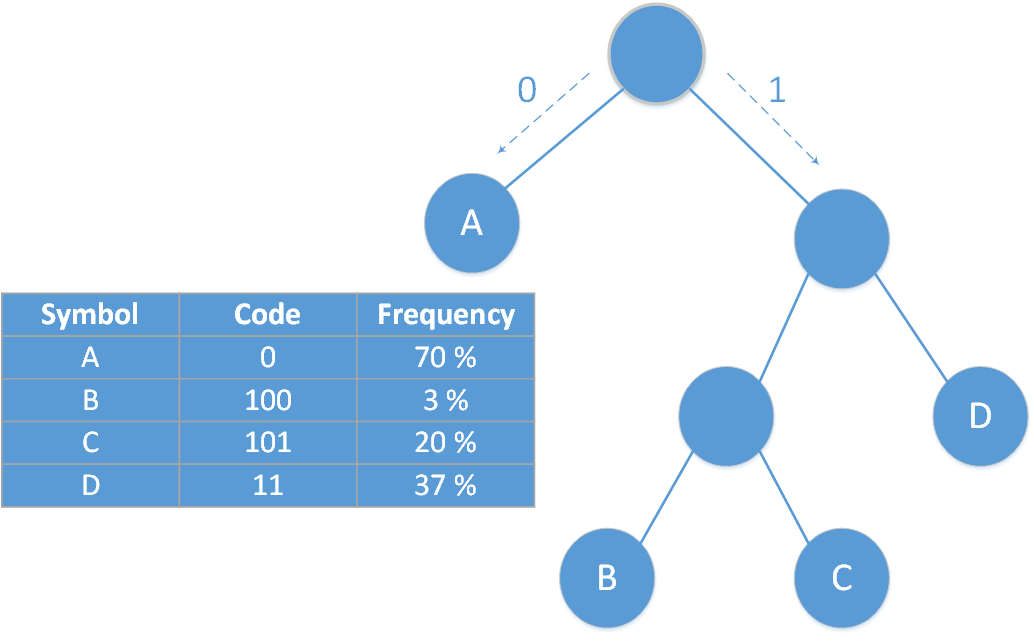
\includegraphics[width=1.0\textwidth]{images/huffman.png}
		\caption{Huffman tree with four symbols.}
		\label{fig:hm-ex}
\end{figure}

\paragraph{}
In the context of compressing data coming from the detector there is one particular foreseen complication.
First of all, generating the Huffman tree needs values from the detector, so how do one create a tree with high compression factor without knowing this?
One answer to this is to generate a tree using existing data from previous experiments, but update the tree when receiving new data.
This gives us an uncertain compression factor in the beginning, but it will become better over time.
Because of a shifting baseline encoding the signal values directly may lead to a large Huffman tree, and the best tree for one channel may not be the same for another.
It is inefficient to create a separate tree for each channel, as there will be 160 channels for every \gls{fec}.
A possible solution to this is to encode the derivative of each signal in a time frame compared to the previous value.
In other words, for every signal \textit{n} you store the value: \textit{signal(n) - signal(n - 1)}.
Doing so takes away the problem caused by shift in the baseline as it only stores the difference between two signals.
This method requires that the first value of every time frame is stored somewhere(maybe the header of a \gls{sampa} packet) in order to decode it later on.


\paragraph{}
The way the \gls{fifo} buffers for each \gls{sampa} channel works is that it stores up to 10 bits in parallel for each slot.
This means that compressing 10 bit samples into smaller sizes will still take up 10 bit of space in the buffers. 
However reading the data from the buffer will be faster as there is less data to read.

\section{Designing the simulation model}
With all of the information regarding the different components already specified, creating a simulation model should be more than feasible.
There will be in total 3 main modules part of the simulation: the \gls{sampa}, \gls{gbt} and \gls{cru}, but the thesis will focus heavily on the \gls{sampa}, leaving the \gls{gbt} and \gls{cru} mostly empty as what happens after data leaves the \gls{sampa} is outside the scope.
In addition to the different modules there is need for a module which can be tasked with producing and/or distributing sample data to the simulation.
This module will contain all methods of sending samples to the different \gls{sampa} channels and in doing so start the entire simulation process.
The tasks, objectives and goals that this all boils down to is summarized in the list below.

\begin{itemize}
	\item \textbf{Tasks}
		\begin{itemize}
			\item Designing a model which is accurate, simple and customizable.
			\item Creating a data generator module which can send data to the simulation, both synthetic and real.
			\item Create a simulation test bench that allows for quick changes in order to run multiple simulations.
			\item Run different stress tests on the system, find out where it breaks and why.
			\item Run focused simulations on the \gls{sampa} channel buffers.
			\item Run simulations which compares \gls{zs} and Huffman encoding.
			\item Gather, and compile the simulation data into a readable and understandable format.
			\item Verify that the simulation results is comparable to what is expected, and calculated beforehand.
		\end{itemize}
	\item \textbf{Goals}
	\begin{itemize}
		\item With a verified simulation model, we have a created a strong argument that the results are valid.
		\item Find out how much \gls{sampa} buffer space is needed.
		\item Conclude the compression factor of both \gls{zs} and Huffman encoding.
		\item Verify the overall design of the \gls{sampa} chip, and use the results to come with a recommendation on possible changes.
	\end{itemize}
\end{itemize}

\section{Workflow}
Approaching this project, one must assume that there will be many uncertainties along the way.
Trying to simulate behaviour of an electronic system based solely on its early schematics, while others are working on the design in different areas will undoubtedly lead to many changes in the simulation model.
Another characteristic concerning this project is that it requires a lot of work before one can start to see any results, but after completing a satisfying  model the results should be easy to obtain without many changes to the simulation program.
Splitting the work into different phases, first a longer period of only working on the model, implementing the aspects that are known, and making the model ready to run simulations on.
When the base model is complete, an iterative process can start.
Simulate for a specific scenario, gather results from the simulation, compile it into a readable format, verify the correctness of the results, in the case they are not legitimate, make adjustments before running new simulations in the same scenario.
Customize the simulation parameters and tweak the model for different scenarios, and do the same as before.
This way any changes in requirements, or changes to the model can be handled in a separate iteration.
Working like this will result in a large period with no speakable results, but this will towards the end be very beneficial.

\chapter{Solution implementation}
\textit{Code snippets, Incremental implementation stages and the final implementation, (before and after huffman), using real data vs random. Implementing fluxiation into the simulation}
\section{Implementing the model in SystemC}

\subsection{The SAMPA module}

\paragraph{•}
As the focus of study in this project, the implementation of the \gls{sampa} module is the most important piece to the simulation.
The overall structure to the \gls{sampa} consists of 32 channels, with an input port for each channel, and in total 4 serial outputs which reads data from the channel buffers.
There are a couple of things to think about when translating this design into code.

\begin{enumerate}
	\item What \gls{sc} channel should the input and output ports use.
	
		\begin{itemize}
		\item The requirements for the \gls{sampa} I/O ports is that everything comes in the correct order, and on a specific clock cycle.
		\gls{sc} comes with the channel type \codeword{sc\_fifo}, it contains both read and write methods, depending on what channel interface is implemented.
		So for our one directional design this should work perfectly.
		The clock cycle is not tied to the ports specifically and will be handled separately.
		\end{itemize}	
		
	\item What data structure to use for the channel buffers.
		\begin{itemize}
\item When choosing a data structure one need to think about what the purpose of it is, what operations are being done on it, and so forth.
		The essential attributes the structure must have are: \textit{Insert} items to the back, \textit{Read/Remove} items from the front, dynamical storage space, and the structure should be a linear one-dimensional sequential storage.
		At first glance using a \gls{fifo} like structure sounds like the best way to go.
		However in addition to the essential attributes it may be needed to be able to remove and read from the back of the buffer.
		This is important, as it allows the system to grab statistical data from the buffer, and read operations won't have any impact on the simulation result, but instead can make the buffers more versatile.
		\gls{cpp} has many different data structures to choose from, all depending on the need for it.		
		In \ref{tab:ds} three different \gls{cpp} data structures are being evaluated: \codeword{vector}, \codeword{list} and \codeword{queue}.
		From this table and the requirements of what is needed from the buffer structure, it becomes clear that the \codeword{list} container has all the attributes needed, as well as performing equally or better than the rest in the different operations.
\end{itemize}
	\item Handling the clock frequency.
		\begin{itemize}
		\item \gls{sc} will handle the clock frequency for us, the only thing to note is that \gls{sc} uses pauses in the threads as a way to simulate the clock cycles.
		In other words, one perform the actions for one clock cycle, then execute the wait statement, and repeat.
		This means that the frequencies need to be converted to a time delay.	
		An example of such a conversion is shown in listing~\ref{lst:cons-ex}.
		\end{itemize}	
	
\end{enumerate}

\begin{table}[bh!]
\begin{tabular}[h!]{| l | l | l | l | p{6cm} |}
\hline
 & \multicolumn{3}{c |}{\textbf{\large{Time}}} & \\
 \hline
\textbf{Operation} & \textbf{Vector} & \textbf{List} & \textbf{Queue} & \textbf{Remarks} \\
\hline
Add back & O(1) & O(1) & O(1) & Constant time for all containers.\\
\hline
Add front & O(n) & O(1) & X & Vector does not have a direct method for adding to front. Queue cant do that at all.  \\
\hline
Access back & O(1) & O(1) & O(1) & Constant time for all containers.\\
\hline
Access front & O(1) & O(1) & O(1) & Constant time for all containers.\\
\hline
Remove front & O(n+m) & O(1) & O(1) & Vector erase is linear to number of deleted elements + number of elements after last deleted item (moving). \\
\hline
Remove back & O(1) & O(1) & X & Queue does not have a method for doing this.\\
\hline
Size of container & O(1) & O(1) & O(1) & Constant time for all containers.\\
\hline

\end{tabular}
\caption[Data structure comparison]{Data structure comparison\cite{vector}, \cite{list}, \cite{queue}.}
\label{tab:ds}
\end{table}

\paragraph{•}
The setup for the \gls{sampa} uses a single thread for receiving signals, and four individual threads which represents the serial outs.
It also stores the channel header and data buffers in two separate arrays, declaring input ports, and the output eLinks.
Let's look at how the implementation for receiving signals can look like.
In listing~\ref{lst:sampa1.2} the thread logic is implemented, and already some weaknesses with the \gls{sampa} module becomes clear.
Having to iterate over every channel every timebin can become costly and hard to maintain when the code becomes more complex.
In the code shown there is already a flaw, if one of the channel buffers has \codeword{overflow}, none of the other buffers will receive data.
The \codeword{overflow} variable needs to be stored as an array to be able to know what channel it represented.
The same problem will occur for every other variable that is unique for each channel.
A principle of \gls{oop} is single-responsibility, meaning that every class/object should be responsibly for one piece of functionality\cite{martin2011agile}.
One solution to the previous problem following this principle can be to create a \codeword{Channel} sub-module inside of the \gls{sampa} module.
The \codeword{Channel} module will contain logic for receiving signals, as this happens for every channel, while the \gls{sampa} will contain the serial outs, which are accessing data from the buffers.

\begin{minipage}{\linewidth}
\lstinputlisting[caption=Sampa receive thread.,firstline=27,lastline=48,label=lst:sampa1.2]{codelistings/sampa1.cpp}
\end{minipage}

\paragraph{•}
The corrected overall structure for the \gls{sampa}, and the new \codeword{Channel} module is shown in Appendix~\ref{cha:app-code}.
As seen there the \gls{sampa} now has an array of \codeword{Channel} modules, a new method called \codeword{initChannel()} that initiate the channels, and connects them to the correct input port.
The \codeword{Channel} module now has the \codeword{receiveData()} thread, and its own data/header buffer.
Having it structured like this makes it possible to add \codeword{Channel} specific variables or methods, without disturbing the \gls{sampa} as a whole.
The implementation of the receive thread is now more simple in terms of complexity, and is exclusive for each \codeword{Channel}.
Listing~\ref{lst:receive-channel} shows the basic thread structure, excluding any data compression or processing.
It continuously receives samples and adds them to the buffer, unless the buffer reach its maximum size.

\begin{minipage}{\linewidth}
\lstinputlisting[caption=New version of the \gls{sampa} receive thread now implemented in the Channel sub-module.,firstline=26,lastline=57,label=lst:receive-channel]{codelistings/channel.cpp}
\end{minipage}

\paragraph{•}
The implementation of reading from the buffer is somewhat more complicated than receiving data.
This is because the real reading procedure is more complex in itself.
In listing~\ref{lst:read-buffers} the most important parts of the code implementation is shown.
The procedure loops through the eight channels for the given serial out, getting the correct channel, and reading out the entire time frame.
This procedure is ran for all four serial out threads at the same time.
One thing to notice here is that the actual data from the buffers aren't passed along further.
This is because we only care about the time it takes to transfer them, which is being calculated in the \codeword{wait} statement.
The header packet is sent as it contains important information which can be useful later on.

\paragraph{•}
\begin{minipage}{\linewidth}
\lstinputlisting[caption=Reading data from the SAMPA buffers.,firstline=28,lastline=58,label=lst:read-buffers]{codelistings/sampa2.cpp}
\end{minipage}

\subsubsection{Implementing Zero Suppression}

\paragraph{•} 
Now that the input channels, and the serial outs are in place, the data processing can be implemented.
The \gls{zs} occurs before the samples are added to the channel buffers, so the correct place to put it in the simulation will be in the \codeword{Channel} module's \codeword{receiveData()} method.
Since this is a piece of code which needs to be turned off and on, the implementation is done in its own method called \codeword{zeroSuppress}.
The method needs the current sample, the last received sample, and some meta-data about the current behaviour of the time frame.
The rules for the \gls{zs} is described in detail in section~\ref{subsec:zs}, therefore this section will only look at the implementation.

\paragraph{•}
By looking at the two last samples the \codeword{Channel} received, the \gls{zs} algorithm can do one of four things depending if they the samples are over or under the \gls{zs} threshold.
In code this translates to four different conditional statements, in this case the implementation uses \codeword{if-else} statements, as seen in listing~\ref{lst:zs-ifelse}.

\paragraph{•}
\begin{minipage}{\linewidth}
\lstinputlisting[caption=If-else structure for the Zero Suppression algorithm.,firstline=1,lastline=10,label=lst:zs-ifelse]{codelistings/zero-suppression.cpp}
\end{minipage}

\paragraph{•}
When both of the two last samples are over the threshold, the algorithm knows for sure that a valid cluster are found, and marks it as such.
If the current sample is valid, but the last is not, then it isn't clear if the sample is part of a valid cluster, so it is added to the buffer, but marked as invalid for now.
If the last two samples where both invalid, it means that either they are just part of some noise, they can be a part of the last valid cluster, or if the next sample is part of a cluster, they can be merged together, forming a single cluster.
Most of the time the last condition will be very straight forward, but there exists one edge case which makes it more complicated to implement.
The edge case occurs when the last couple of signals has a particular shape.
The problematic sequence is displayed in \ref{fig:zs-prob}.

\begin{figure}[h!]
	\centering
		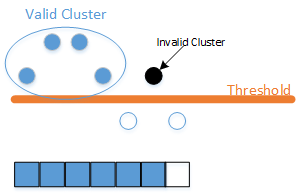
\includegraphics[width=0.75\textwidth]{images/zs-prob.png}
		\caption{An edge case that the Zero suppression needs to handle.}
		\label{fig:zs-prob}
\end{figure}

\paragraph{•}
Now the last sample, which was added to the buffer turned out to be an invalid cluster, and needs to be discarded.
The algorithm must then remove it, and replace it with an empty sample as part of the previous clusters meta-data.
The final implementation of the \gls{zs} algorithm is shown in listing~\ref{lst:zs}.
Since the code was implemented in its own method, all the change needed in the \codeword{receiveData()} thread is to call the \codeword{zeroSuppress()} method instead of adding samples directly to the buffer.

\begin{minipage}{\linewidth}
\lstinputlisting[caption=Zero suppression algorithm.,firstline=12,lastline=44,label=lst:zs]{codelistings/zero-suppression.cpp}
\end{minipage}

\subsubsection{Implementing Huffman encoding}

\paragraph{•}
Huffman is a well known, and widely used algorithm.
Because of this, there are multiple providers which has made the implementation available online for people to use.
The Huffman code used in the simulation is based on code provided by Rosetta Code, licensed under GNU Free Documentation License 1.2\cite{rosetta}\cite{gnu}.
The code is modified slightly to suit the requirements of the simulation program.
In addition methods for writing a full Huffman tree to a file, as well as reading a tree from a source file is implemented.

\paragraph{•}
The simulation will only be able to use the Huffman encoding when it uses realistic data, i.e where the samples have realistic values.
Only when there is a wide spectre of different values can the simulation determine an accurate compression factor.
There are two different sets of realistic data available for use, and they are described in more detail in section~\ref{subsubsec:real-data}.
The Huffman tree will be created directly from the dataset that is used, and saved to a file so that it can be used to decode the samples later on.
Creating the tree in such a manner means that it gets the optimal compression possible.
In the real world a perfect compression is not plausible as signals coming from the detector will continuously change, and it doesn't contain a steady pattern.
Even though using the optimal compression in the simulation doesn't give us the worst case, it can still establish a base estimate that is reasonable.

\subsection{The DataGenerator module}
\paragraph{•}
The simulation model is scoped to the readout electronics, which doesn't handle the creation of signals.
This means that the simulation needs a module which can create and distribute data, both simulated and real to the \gls{sampa} modules.
The module needs to be able to continuously send samples based on what is desired for a specific simulation scenario.
It is important that all the different methods for sending samples, do so in the same fundamental way.
The rest of the simulation model should not need to change for each different scenario, but instead the data generator should make sure that it sends samples in the correct format, regardless of the simulation type.

\paragraph{•}
With the expected behaviour given in the previous paragraph, the bounds and requirements of the data generator can be established.
The module will continually be updated, and new functionality will be added as new simulation scenarios surface. 
In order for this to be efficient, the module needs to be easily extended, without causing any disturbance to the rest of the module.
Sending samples should follow the specifications for the actual hardware, emulating the connection between the readout chambers and the \gls{sampa} asic.
That includes the clock frequency and making sure every channel receives data asynchronously.

\subsubsection{Basic data generating functions}

\paragraph{•}
Achieving the same format for every simulation sample is done by using a custom class which forms the link between the data generator and what the \codeword{Channels} are expecting as input.
This means that every time the data generator sends a signal it uses this class.
The format of the \codeword{Sample} class is discussed and shown in section~\ref{subsec:signal-classes}.
Creating a single function that has the core functionality of data generator, which all simulation scenarios used as base could have been a good way to remove some of the boilerplate code needed, but without knowing all types of simulations from the start this could lead to unwanted restrictions later on.
Because of this, for every different way of creating/distributing data, there is a completely different function.
The benefits of implementing it like this is that the functions does not depend on each other and can be separately updated or improved, which allows for easier development as the module becomes larger and more complex.

\paragraph{•} 
To be able to quickly switch between different functions when running a different simulation, the module contains only a single \gls{sc} thread, where it is possible to choose the correct function based on the simulation type.
The \codeword{sink\_tread()} function can be seen in listing~\ref{lst:sink-thread}.
In listing~\ref{lst:sink-thread} the variable \codeword{DG\_SIMULATION\_TYPE} is used.
This variable is stored in what is referred to as the simulation testbench.
Throughout the following code listings many variables from the testbench will be used.
In short the testbench is a \codeword{class} which defines a global \codeword{namespace} where every shared variable or property for all modules part of the simulation is stored.
The testbench makes it very easy to run multiple different simulations in quick succession.
In most cases this will be the only file which is modified in between simulations, only changing the properties the simulation uses.

\begin{minipage}{\linewidth}
\lstinputlisting[caption=Data generator SystemC thread.,firstline=1,lastline=13,label=lst:sink-thread]{codelistings/dg.cpp}
\end{minipage}

\paragraph{•}
They have been implemented one by one in different stages of the development phase.
The first three: \textit{standardSink()}, \textit{incrementingOccupancySink()}, and \textit{alternatingOccupancySink()} are functions created in the early stages, before there was any need to implement compression schemes in the simulation model.
They all assume that the data being generated are already compressed, and can be sent through the simulation without any data processing.
The shear amount of samples is the important factor with these functions, relying on a flat occupancy value to determine if a sample is sent.
The chosen occupancy(specified as percent(0-100)) is compared against a number generated by a \gls{rng}.
If the number is lower then the occupancy the sample is sent, else it will send an empty sample instead.
In other words, a sample is sent a fixed percent of the time, specified by the occupancy.
The \textit{standardSink()} implementation is shown in listing~\ref{lst:standard-sink}.
The double loop seen here is just about the same for all the five functions, where the outer one counts the number of time frames and the inner goes through all \gls{sampa} channels present.
The wait statement is called after the inner loop, which is equivalent to sending samples to all channels in the same clock cycle.
This function is a good starting point in order to test the rest of the simulation model, and to verify that the model can be trusted.
Since it relies on a flat occupancy it is expected that most channels will get similar data, and there will be little to no fluctuations.
Real experiment data will not be as flat, and the occupancy will differ from time frame to time frame.

\begin{minipage}{\linewidth}
\lstinputlisting[caption=Data generator SystemC thread.,firstline=15,lastline=37,label=lst:standard-sink]{codelistings/dg.cpp}
\end{minipage}

\paragraph{•}
The limitations of the \textit{standardSink()} function was the motivation behind the \textit{incrementingOccupancySink()} and the \textit{alternatingOccupancySink()}.
As their names suggest they implement more diversity into the simulation with the ability to increase, or alternate the data occupancy as time goes.
This creates more possibilities to test the limits of the model, especially the \gls{sampa} buffers.
The code for these functions is similar to the \textit{standardSink()}, and the differences is shown in listing~\ref{lst:sink-diff1} and listing~\ref{lst:sink-diff2}.

\begin{minipage}{\linewidth}
\lstinputlisting[caption=Difference between standardSink() and incrementingOccupancySink() functions.,firstline=1,lastline=17,label=lst:sink-diff1]{codelistings/dg-diff.cpp}
\lstinputlisting[caption=Difference between standardSink() and alternatingOccupancySink() functions.,firstline=20,lastline=32,label=lst:sink-diff2]{codelistings/dg-diff.cpp}
\end{minipage}

\paragraph{•} 
The \textit{incrementingOccupancy()} will provide initial results on how much occupancy the system will be able to handle, while the \textit{alternatingOccupancySing()} will test its ability to handle various amount of data distributed over time.
This is an improvement from the \textit{standardSink()}, but the functions do still not care about how the data is shaped or distributed inside a time frame.
To get more accurate results from the simulation there is a need for data which more closely resembles actual experiment data.
The implementation so far doesn't worry about the value of the samples, but the values are required in order to test \gls{zs} and Huffman encoding.

\subsubsection{Creating Normally distributed samples}
\label{subsubsec:normal-distribution}
\paragraph{•}
Measured occupancies gathered from experimental events recorded in 2010 provides a graph of expected average occupancies within a time frame.
This is shown in \ref{fig:expected-occupancy}, where the x axis is the position of a pad row on the actual detector.
The closer to origin, the closer to the center of the detector.
The pads closer to the center has generally higher occupancy than the outer ones, which makes them the worst case, and the most interesting for use in the simulation.
\ref{fig:expected-occupancy} shows that the average occupancy for the inner pads is 28\%, but it can reach 44\%, or with a high multiplicity as high as 74\%.
The chance of reaching a multiplicity equal to 44\% occupancy is 10\%, while only 1\% chance to reach 75\%.
Based on this a normal distribution of occupancies can be created for a more realistic simulation.
A normal distribution is a mathematical/statistical distribution of values which depend on a central value (the mean value) and a stretch factor (the standard deviation)\cite{normal-dist}.
The formula for a normal distribution is as followed: $f(x,\mu,\sigma) = \frac{1}{\sigma}\phi(\frac{x-\mu}{\sigma})  $, with $ \mu$ being the mean value and $ \sigma$ the standard deviation. 
An example of a normal distribution is shown in \ref{fig:normal-dist}

\begin{figure}[h!]
	\centering
		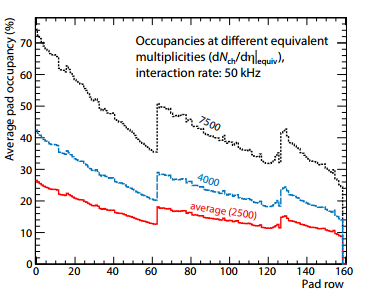
\includegraphics[width=0.5\textwidth]{images/expected-occupancy.png}
		\caption[Expected average occupancies within a given time frame.]{Expected average occupancies within a given time frame. \cite{tdr-016}}
		\label{fig:expected-occupancy}
\end{figure}


\begin{figure}[h!]
	\centering
		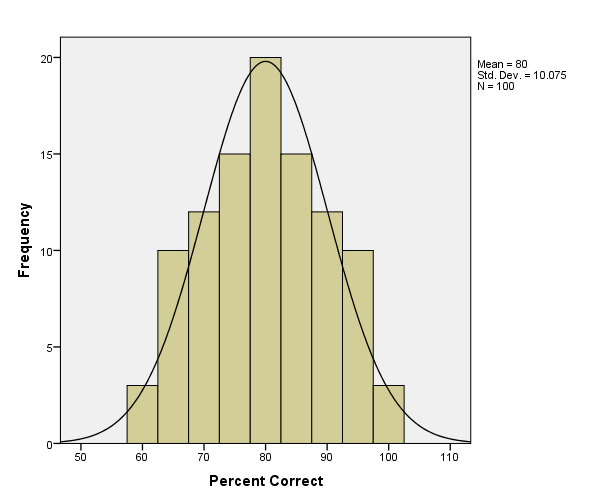
\includegraphics[width=0.6\textwidth]{images/normal-dist.png}
		\caption[Normal distribution.]{Normal distribution. \cite{normal-dist-image}}
		\label{fig:normal-dist}
\end{figure}

\paragraph{•}
Using a normally distributed \gls{rng}, a set of occupancy values can be created.
For every new time frame in the simulation, a random value from the set is picked as the current occupancy.
The size of the set is determined by the number of time frames in the simulation.
The mean value for the distribution is already known being 28\%, but the standard deviation is not obvious and needs to be calculated.
Using the statistics given in \ref{fig:expected-occupancy} the deviation can be calculated.
In a set $x$ of 100 values, 1 value will be 74, 10 will be 44 and the rest will on average be 28.
First of the \textit{variance} must be calculated by the following formula:
$ \frac{\sum_{i=1}^{100} (x_i - mean)^2}{100}$
Take the square root of the \textit{variance} and the result is the standard deviation.
How this is implemented programmatically is shown in listing~\ref{lst:standard-deviation} along with creating the final set of occupancies.

\paragraph{•}
\begin{minipage}{\linewidth}
\lstinputlisting[caption=Data generator SystemC thread.,firstline=40,lastline=62,label=lst:standard-deviation]{codelistings/dg.cpp}
\end{minipage}

\paragraph{•}
After testing the distribution out the conclusion was that the distribution became very narrow towards the mean.
By using values from $mean-10$ to $mean+10$ gave a bigger deviation, and as a result a wider distribution.
A wider distribution will most likely create more interesting results.
The difference by increasing the deviation is shown in \ref{fig:distribution}.

\begin{figure}[h!]
	\centering
		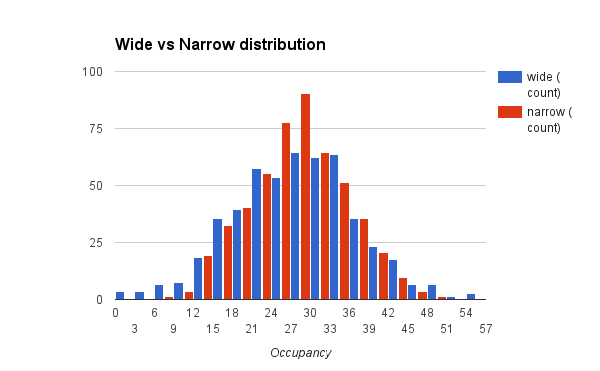
\includegraphics[width=1.0\textwidth]{images/normal-dist-diff.png}
		\caption{Difference in the normal distribution.}
		\label{fig:distribution}
\end{figure}

\paragraph{•}
To be able to test the \gls{zs} the samples need to have a shape which allows for this.
The \gls{zs} works best with data where the peaks are wider, but further apart from each other.
So to test it in its worst case the samples the time frame need to have as many peaks as possible, split evenly over it.
A peak will be of width 3, and the occupancy for the time frame determines the space between two peaks.
An example using 28\% occupancy is displayed in \ref{fig:normal-data-shape}.
Even though the data still doesn't look like the real thing, in the case of testing the \gls{zs} it should sufficient since it only cares if the sample value is zero or above.

\paragraph{•}
A process for determining the space between each peak is the next thing to look at.
The space can be calculated by first finding the number of samples with value 0, and divide it by the number of peaks in the time frame.
Since both the occupancy and the number of samples in a time frame is known, the math becomes very straight forward.
The solution used is shown in listing~\ref{lst:calc-space}.

\begin{figure}[h!]
	\centering
		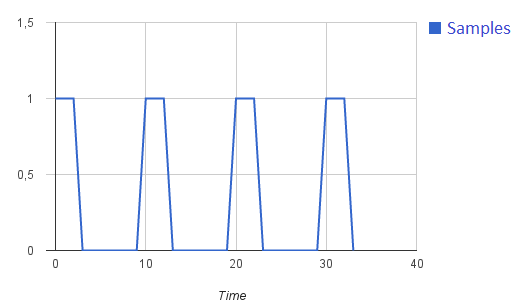
\includegraphics[width=0.75\textwidth]{images/normal-data-shape.png}
		\caption{FEIL FIGUR!}
		\label{fig:normal-data-shape}
\end{figure}

\paragraph{•}
\begin{minipage}{\linewidth}
\lstinputlisting[caption=Calculating the space between two peaks in a time frame.,firstline=64,lastline=70,label=lst:calc-space]{codelistings/dg.cpp}
\end{minipage}

\paragraph{•}
With a completed set of occupancies and the necessary functions to help shape the data the only thing left is to implement the sink function.
It uses the same loop structure as the three previous sink functions, but in addition before every new time frame it picks the next occupancy from the set.
Then using the current occupancy to calculate the number of empty samples between the peaks, and starts sending the samples in the correct order.

\subsubsection{Realistic datasets}
\label{subsubsec:real-data}

\paragraph{•}
The last type of simulation will use realistic datasets as input. 
Two types of datasets have been available for use: Black event data collected from RUN 1, and synthetic data created by researchers which matches the expected data from RUN 3.
Black events is the term for when there is data in all channels at the same time, which means overall higher occupancy then normal events.
In addition to this, we want to use the data from RUN 1 and create pileup data.
Pileup occurs when a channel gets overlapping data from multiple neighbouring channels in the same time frame.
In the worst case the pileup can happen five times, i.e samples from five neighbouring channels are causing interference.
By overlapping five time frames from the RUN 1 data, a third set for use in the simulation is made available.
For the sake of clarity the datasets will be noted as: black-events, synthetic and pileup data from now on.
 
\paragraph{•} 
The format for the black-events and the pileup datasets are as followed:
\begin{minipage}{\linewidth}
\begin{lstlisting}[caption=Format for the black-event and pileup dataset., label=lst:black-event-format]
ddl <ddl number>
hw  <hardware addr>
<start time> <time frame length>
<timebin> <signal>
<timebin> <signal>
....
hw <hardware addr>
\end{lstlisting}
\end{minipage}

\paragraph{•}
The hardware address is a decimal number which represents the channel, the \gls{altro} chip, the front-end card and branch address.
Even though it is displayed as a decimal, it can be translated into four different values using bitwise operators.
The bitwise operation looks as following: $BranchNr << 11 | FecNr << 7 | AltroNr << 4 | ChannelNr $.
In \ref{fig:hw-binary} an example address is shown, displayed in binary and the bits representing each of the four values are highlighted.
In this context the ddl number is not important, but ddls with low numbers usually has a higher than average occupancy among its channels.

\begin{figure}[h!]
	\centering
		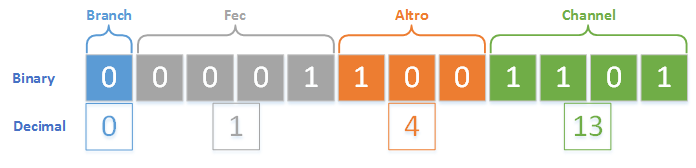
\includegraphics[width=1.0\textwidth]{images/hw-binary.png}
		\caption{Example hardware address(205) in binary, with translated addresses below.}
		\label{fig:hw-binary}
\end{figure}

\paragraph{•}
To get the different values from the original hardware address, the opposite bit operation than the one used to store it is applied.
Taking the \textit{BranchNr} as an example.
Its value is stored by taking the value and left shifting it 11 bits, so in order to reverse it all that is needed is to right shift the hardware address 11 bits.
\paragraph{•}
\begin{minipage}{\linewidth}
\begin{lstlisting}[caption=Bitwise operation to retrieve values from the hardware address., label=lst:bit-operation]
int BranchNr = (hw >> 11);
int FecNr = (hw >> 7) & 15;
int AltroNr = (hw >> 4) & 7;
int ChannelNr = hw & 15;
\end{lstlisting}
\end{minipage}

\paragraph{•}
The formatting used for the synthetic data is more straight forward then the one for black-events.
It starts with one row with the title of values in its column, before continuously storing rows of data, following the format specified in the first row.
The main difference between the two formats is that the synthetic stores the exact pad and pad row for every timebin, instead of storing it before the start of every time frame, as in the black-events.

\begin{lstlisting}[caption=Format for the synthetic dataset., label=lst:synthetic-data-format]
#sector #padRow #padNr #timebin #signal #meta-data
\end{lstlisting}

\paragraph{•}
The next step is creating a shared data container which can store samples from any dataset, this way the simulation only needs one sink function.
The data container needs to store samples for every channel, and for every time frame that is being simulated.
This can be made by defining a simple \codeword{template} using existing containers.

\begin{lstlisting}[caption=Data container., label=lst:data-template]
typedef std::map< int, std::list<Sample> > DataEntry;
typedef std::vector< DataEntry > Datamap;
\end{lstlisting}

\paragraph{•}
The \codeword{DataEntry} template stores one entire time frame worth of samples for every channel in the simulation.
The \codeword{Datamap} is just a \codeword{vector} storing \codeword{DataEntry} objects.
One weakness of storing the samples in this manner is that the sink function will now expect that it contains full time frames for all channels.
In other words, it expects that the datasets contain 1022 signals for every channel, which is not the case.
The black-event data was based on the \gls{altro} chip, meaning there is only 8 chips per front-end card, and 16 channels per \gls{altro}.
At the same time the time frame seems to be shorter, so there is always less then a full time frame worth of data.
The lack of samples can easily be fixed by placing empty samples at the front and/or back of each time frame.
Doing so will create full time frames no matter the actual number available.
Regarding the channel mismatch in the black-event data, it can be remedied by creating a mapping table, using neighbouring channels to fill in the gap.
Even though there is enough channels to work with, the dataset still only contains three time frames worth of data for each channel used in RUN 1.
Three time frames is not enough to create valid results, which means that data from other channels need to be used as well to create longer simulations.
Since the current solution still proposes to use a fake mapping between \gls{altro} and \gls{sampa} channel, why not read in data without caring about which channel it belongs to.
Doing so will provide more then enough time frames, and since these are black events, the occupancy should be on average the same non the less.

\paragraph{•}
The synthetic data has a mapping which is usable for the \gls{sampa} channels, but only contains 1000 signals per time frame.
As with the black-event data, the lack of samples is solved by placing empty ones where it is needed.
There is more then enough synthetic data to use, but since it stores time frames for every single pad in the readout chamber reading out a meaningful amount of time frames for the same channels will be very time costly.
The only alternative is to disregard the mapping, and focus on reading in data instead.

\begin{figure}[h!]
	\centering
		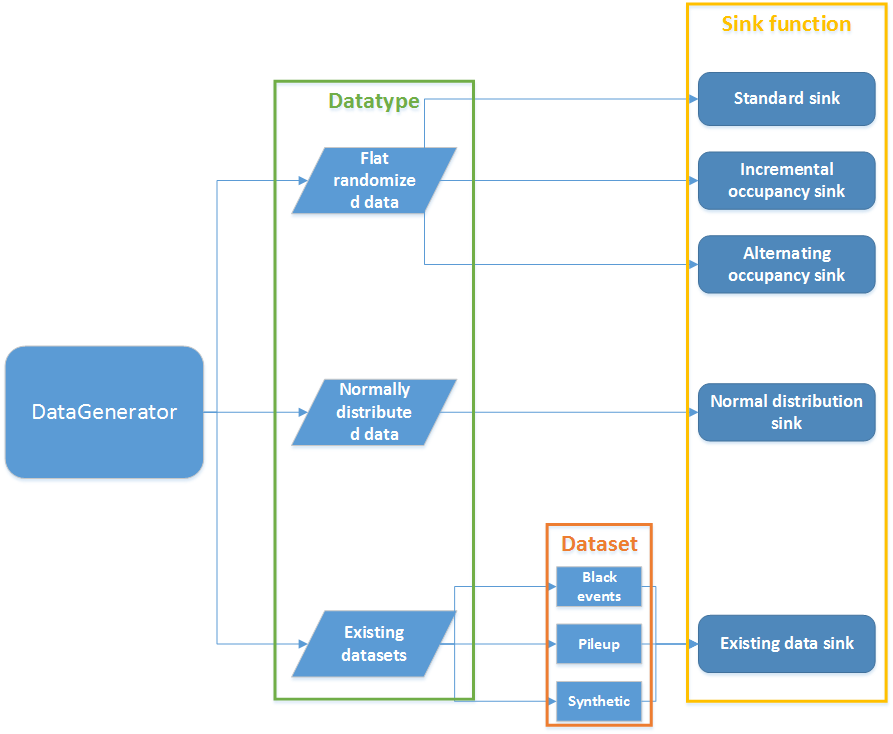
\includegraphics[width=0.75\textwidth]{images/dg-overview.png}
		\caption{Overview of the different data sources and sink functions in the DataGenerator.}
		\label{fig:dg-overview}
\end{figure}

\paragraph{•}
With three different data sinks which uses a flat occupancy, a more advanced data model using normal distribution, and three different sets with realistic data, the simulation is sure to provide some interesting results.
The different simulation types, and sink function being used are all displayed in \ref{fig:dg-overview}.

\subsection{Signal classes}
\label{subsec:signal-classes}
\paragraph{•}
\gls{sc} allows the creation of custom \codeword{classes} to be used as data type when transferring data between modules.
There are some requirements when doing so that needs to be fulfilled for it to work.
\gls{sc} requires you to define several methods which is vital for the read/write methods of a \gls{sc} channel.
The read/write methods involve copying the custom data type.
Because of this it requires the definition of the assignment operator(\codeword{operator=()}).
In addition the output streaming(\codeword{ostream\& operator<<()}) method is required. 

\paragraph{•}
The simulation needs two different data types, these have been briefly shown in the previous code listings.
The \codeword{Sample} and the \codeword{Packet} classes.
\codeword{Sample} represents a single 10-bit signal, storing information about what time frame the sample belongs to, the signal value itself, and other statistical variables.
Representing the \gls{sampa} header is the \codeword{Packet} class, it stores the relevant values selected from its documentation.
This include the time frame, channel id, sampa id, number of samples and whether there was overflow in its time frame.
Source code for the \codeword{Packet} class is shown in listing~\ref{lst:packet}.
The \codeword{Sample} class is implemented in similar fashion and will not be displayed in the report. 

\begin{minipage}{\linewidth}
\lstinputlisting[caption=Custom data type - The SAMPA header.,label=lst:packet]{codelistings/packet.cpp}
\end{minipage}

\subsection{Connecting the modules together}
\paragraph{•}
As seen in chapter~\ref{cha:3} connecting the modules together is done in the \codeword{sc\_main} method.
The implementation becomes a little more complex when dealing with such a large amount of different modules, as well as sub-modules.
In order for the simulation to function correctly the modules must be connected the right way.
The connection occurs in three stages:
\begin{itemize}
	\item Instantiating the modules.
		\begin{itemize}
			\item This is done by simply creating arrays of module objects, iterate that array and instantiate new objects.
			\item The number of modules is specified in the testbench, which makes it possible to easily edit the number of \gls{sampa} chips, or channels per \gls{sampa}.
		\end{itemize}
	\item Initialize the \gls{fifo} channels.
		\begin{itemize}
			\item An array of \gls{fifo} channels must be created for every pair of modules that are connected together.
			\item An overview of the number of channels between each module is shown in \ref{fig:sampa-overview}.
		\end{itemize}
	\item Connecting the modules together.
		\begin{itemize}
			\item In this case the DataGenerator needs to have 32 different channels per \gls{sampa} module, the \gls{sampa} needs four channels to the \gls{gbt} and from the \gls{gbt} to the \gls{cru} one is needed.
			\item So by having three arrays of \gls{fifo} channels, they can be set as channels for the three pairs of modules that needs to be connected.
			\item In listing~\ref{lst:connecting-modules} the connection between the \gls{sampa} and the \gls{gbt} is used as an example.
		\end{itemize}
\end{itemize}

\begin{figure}[h!]
	\centering
		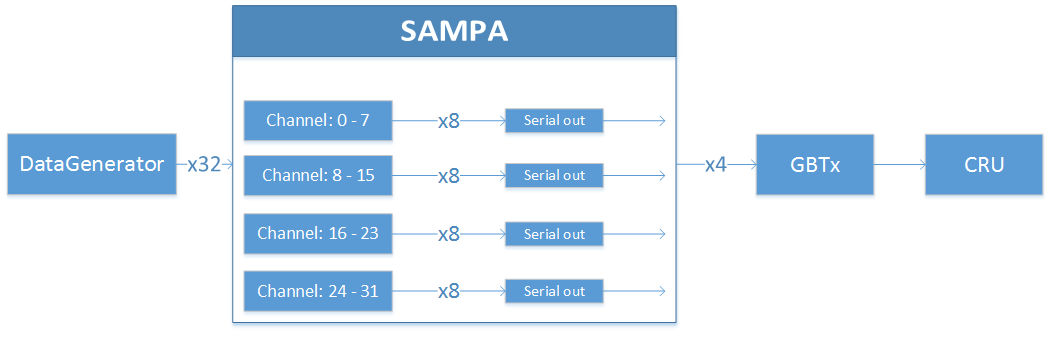
\includegraphics[width=1.0\textwidth]{images/sampa-overview.png}
		\caption{Overview of the number of channels between every module.}
		\label{fig:sampa-overview}
\end{figure}

\begin{minipage}{\linewidth}
\lstinputlisting[caption=Connecting the \gls{sampa} modules with the \gls{gbt}.,label=lst:connecting-modules]{codelistings/connection.cpp}
\end{minipage}

\section{Data gathering}
\textit{Creating Struct object in the sampa and channel modules to gather information, which can be written to a graph file later on}

\paragraph{•}
Taking advantage of the fact that the main method stores every module in memory, they can be accessed after the simulation is done, and simulation data stored in them can be gathered.
The most important modules is of course the \textit{channel} and \textit{\gls{sampa}}, so this section will focus on the data gathering from those components, but the same principle is used for all modules.
Every module has one or multiple \codeword{struct} objects, which stores statistical data which has recorded throughout the simulation time.


\chapter{Evaluation and results}
\textit{Running the tests, results from different tests, Evaluating the final product}

\section{Introduction}
With a completed simulation model in place, blablabla

\section{Results}

\subsection{Verify the Simulation Model}

\subsubsection{Preface}

\paragraph{•}
To begin with, a number of different simulations is run, all with one goal in mind: verifying the simulation model.
Before using realistic data, the model must be tested to see if it behaves as expected.
In order to trust the results provided by the simulations, the simulation model must be dependable, and accurate enough.
Using static input data which only depends on occupancy, will give a controlled environment where the results can easily be predicted beforehand and compared to the actual results.
Doing some test simulations will also flush out any flaws or weaknesses in the way data is gathered, or if any parameters must be changed.

\subsubsection{1. TITLE}
\paragraph{•}
A good place to begin is to run multiple simulations with different static occupancy level.
This will create a wide range of results to use in verifying the simulation model.
To begin with, three different occupancy levels was used, 30, 60 and 90 percent.
Starting small with only eight time frames per simulation, using the entire \gls{fec}, giving a total of 160 channels.
The maximum buffer size is set to 4k * 10 bit for the data buffer and 256 * 10bit for the header buffer.
The purpose of this simulation is to see how the buffers hold up with the expected data occupancy, compared to higher amounts.

\begin{figure}[h!]
	\centering
		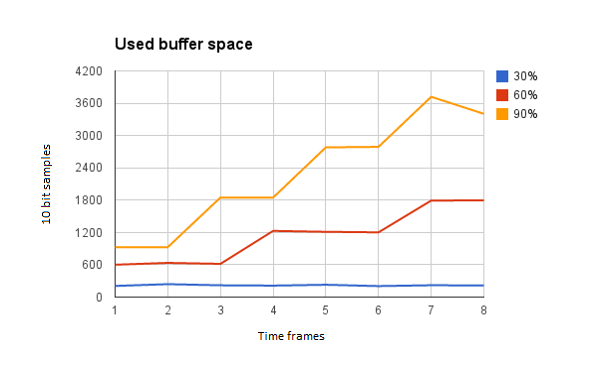
\includegraphics[width=1.0\textwidth]{images/results-flat30-60-80-8tf.png}
		\caption{Comparing buffer usage for three different levels of occupancy.}
		\label{fig:results-30-60-90}
\end{figure}

\paragraph{•} % 50 vs 70 percent 30 tf.
Results from the first simulation were very much as expected.
Given 30 percent the buffer usage remain stable at around 250-300 samples over all time frames, while 60 and 90 percent uses more space as time goes on.
After seven time frames the simulation using 90 percent reaches the maximum buffer usage, causing it to overflow.
From the results one can predict that using 60 percent will also cause overflow, given enough time.
To confirm this prediction, a slightly longer simulation using 50 and 70 percent occupancy is performed.
This time the simulation uses 30 time frames instead of just 8, and the maximum buffer size is set to 8k * 10 bit.

\begin{figure}[h!]
	\centering
		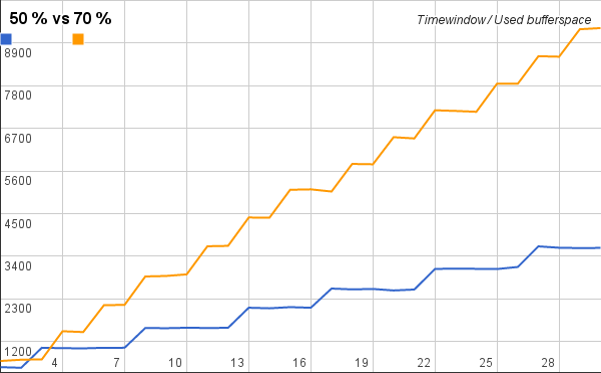
\includegraphics[width=1.0\textwidth]{images/50v70.png}
		\caption{Comparing buffer usage between 50 and 70\% in a longer simulation.}
		\label{fig:results-50-70}
\end{figure}

\paragraph{•} %Sum up
The results confirm the prediction, and it seems that with occupancies higher then 30 percent the buffer usage keeps growing as time goes on, and the serial outs will never be able to read the data fast enough.
Looking at the header buffer during these simulations, it became clear that it will most likely never become full, using only one to two header packets at the most.
This is because it doesn't depend on the data occupancy, every header packet is always 50 bit, no matter how many samples there are in a time frame.
So far the model seems to be working as expected, but the simulation has been using very controlled, and static data.
Some more tests needs to be done in order to confirm that the simulation model is accurate enough to produce valid results with more realistic input data.

\subsubsection{2. Alternating Occupancy}

\paragraph{•} %Intro
The occupancy will in most cases vary from time frame to time frame, and sometimes the won't be any data at all.
Using the \textit{alternatingOccupancySink()} function, a pattern of different levels of occupancies can be used as input.
This way it will be more fluctuations in the amount of input data, which will give more fluctuating results.
The pattern chosen for this simulation is displayed in \ref{fig:occ-pattern}.
It starts off with the expected average occupancy, before increasing in a steep fashion to 100 percent, then more slowly decreases down to zero.
With this pattern, the model is tested how it handles increasing occupancy over time, and how fast it can stabilize after the amount of data decreases.

\begin{figure}[h!]
	\centering
		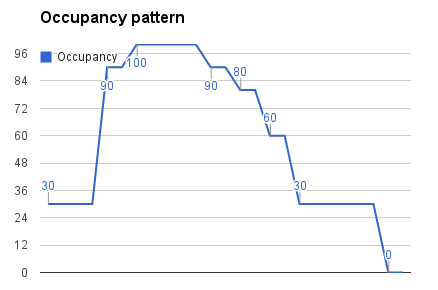
\includegraphics[width=0.8\textwidth]{images/occ-pattern.png}
		\caption{Occupancy pattern used for the simulation.}
		\label{fig:occ-pattern}
\end{figure}

\begin{figure}[h!]
	\centering
		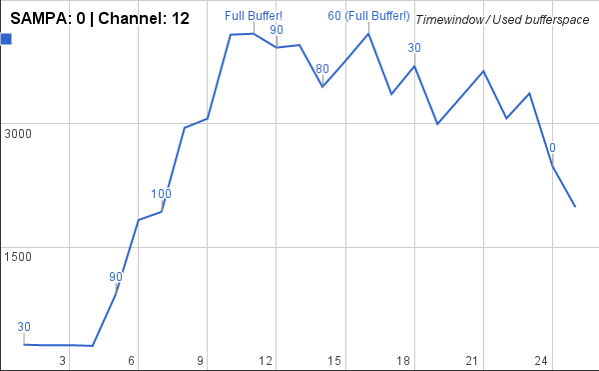
\includegraphics[width=0.8\textwidth]{images/results-alternating.png}
		\caption{Results using a static pattern of occupancies.}
		\label{fig:results-alternating}
\end{figure}

\paragraph{•} %Sum up
Results from \ref{fig:results-alternating} shows that after 10-11 time frames the buffers are already full, but even though the occupancy decreases the serial outs still need more time in order to stabilize.
What is seen is that the resulting buffer usage follows the occupancy pattern, giving more confidence in the model.

\subsubsection{3. Flat 100\% Occupancy}

\paragraph{•} %Intro
This simulation wishes to see how fast the buffer usage increases when getting 100 percent occupancy, as well as seeing how many time frames it takes to reach the estimated 4k * 10 bit size of the buffers.
The expected result is that it will go beyond 4k in the ten time frames being simulated, because of this the maximum buffer size is set to 8k.
The readout speed is 2.5 times slower then the input speed, meaning that every serial out will be able to read around three out of eight channel buffers before the next time frame is finished.
Lets take the first channel as an example: It will be the first channel the serial out will read, and while being read more data will come pouring in.
The channel will have 40 percent of the data from the next time frame already stored when the serial out finish with the first time frame.
Then it needs to wait while the other seven channels are read before coming back to it.
The point here is that the expected behaviour is that the channel buffer usage will rapidly increase, but in small periods it slows down because data is being read out.

\begin{figure}[h!]
	\centering
		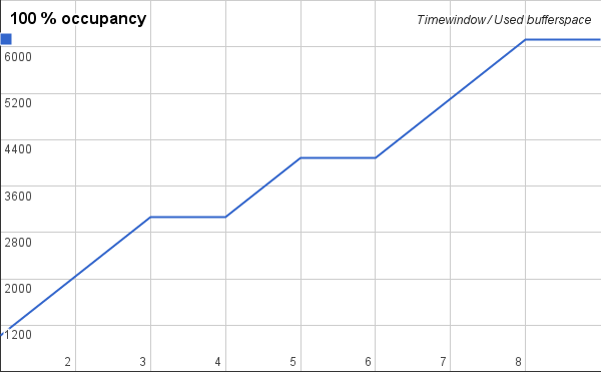
\includegraphics[width=0.9\textwidth]{images/flat-100.png}
		\caption{Results from a specific channel.(Channel 7 on SAMPA 0)}
		\label{fig:flat-100}
\end{figure}

\paragraph{•} %Sum up
The results in \ref{fig:flat-100} shows that the buffer usage increases in a linear fashion until the third time frame.
This means that after three time frames, the serial out started reading from it, which is consistent with the fact that channel number 7 is the last channel read by one of the serial outs.
After five time frames the buffer usage reaches 4k, and it peaks at about 6k after ten time frames.

\subsubsection{4. Increasing Occupancy}

\paragraph{•} %Intro
Some of the problems with the previous simulations has been the length.
They have been too short to be able to say anything for certain.
Improving on this, the next simulation will run for about 100 time frames, with continuously increasing occupancy.
With the high amount of time frames, the resulting graph should provide more detailed information.
Starting ten percent below the expected average of 30 percent, and then increase in a steady fashion until reaching 100 percent.

\begin{figure}[h!]
	\centering
		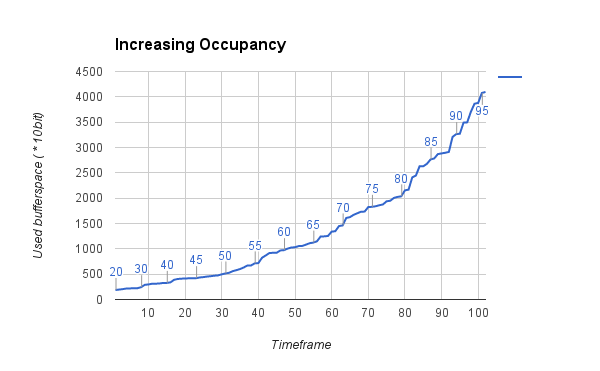
\includegraphics[width=1.0\textwidth]{images/increasing-occ.png}
		\caption{Results using a static pattern of occupancies.}
		\label{fig:increasing-occ}
\end{figure}

\paragraph{•} %Sum up
No real surprises from this simulation, the graph shows a steady increase in buffer usage, which grows faster as the occupancy increases.
This confirms once again that the simulation model is working as intended, and should produce both valid and interesting results.
One thing that was unexpected was the amount of time it took to run the simulation just for one \gls{fec}.
It took about two hours to complete the 100 time frames, and it looked as if the higher the occupancy, the longer it took to complete a time frame.

\subsubsection{Evaluating the Results}

\paragraph{•}
The results from the verification simulations have been very useful when determining how good the model is, but it doesn't really give an indication about the performance of the channel buffers.
This was not the intent of the simulations and to test the performance itself more realistic simulation data is necessary.
In the results from the alternating occupancy simulation it can be seen that every time it reaches the maximum buffer size, overflow occurs and the data from that time frame is removed, causing the graph to decrease slightly.
What was learned from this is that in the future it can be a good idea to remove the buffer size restrictions, in order to see how much is actually used.
Already from the first simulation it became clear that the size of the header buffers won't be an issue, and in future simulations no information about them will be included. 
Regarding the simulation time for longer simulations, it is clear that it needs improvement.
One of the reasons it uses a long time, is that the there are 160 channels to simulate.
If instead only 32 channels, i.e one \gls{sampa} module was used, it would be five times as fast.
Using 32 channels will still give valid results because the simulation doesn't care about what happens after the data leaves the \gls{sampa} module.
This will be implemented for the rest of the simulations, and it can be done without much effort because the testbench stores information about the number of channels.

\subsection{Normal Distribution}

\subsubsection{Preface}

\paragraph{•}
Now that it is established that the model is working as intended, more realistic data can be used as input.
Using the normal distribution sink explained in section~\ref{subsubsec:normal-distribution}, a more accurate estimation of buffer usage can be established.
Another goal of these simulations is finding the compression factor for the \gls{zs}, see how it changes with different levels of occupancy, and where it reaches the necessary factor of 2.5.
The verification simulations showed that simulations of about 100 time frames gave a good amount of data, so the simulations using normal distribution will run at least that long.


\subsubsection{1. 28\% Mean Occupancy}

\paragraph{•}
According to \ref{fig:expected-occupancy} the mean occupancy that is expected is 28 percent, this becomes a natural starting point for the first simulation.
If the results show that the model can't handle 28 percent or it is to little, the occupancy level can be adjusted for the next simulation.
This is what is most likely to happen, because the shape of the data is the worst possible case for the \gls{zs} algorithm. 
In \ref{fig:28-dist} the randomly picked normal distribution used for this simulation is shown.
Values ranging from 0 to 50 percent is being used.

\begin{figure}[h!]
	\centering
		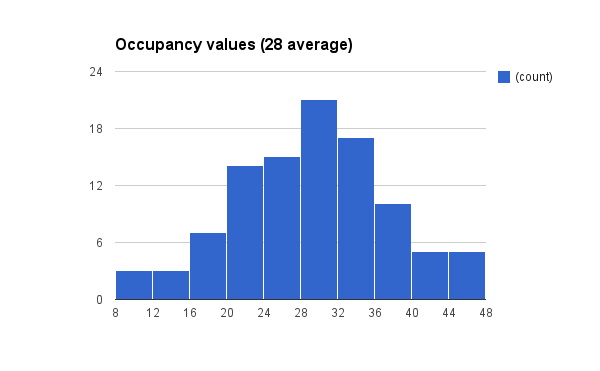
\includegraphics[width=0.9\textwidth]{images/occupancy-28.png}
		\caption{The distribution of occupancies used in the simulation from \ref{fig:28-occ}.}
		\label{fig:28-dist}
\end{figure}

\begin{figure}[h!]
	\centering
		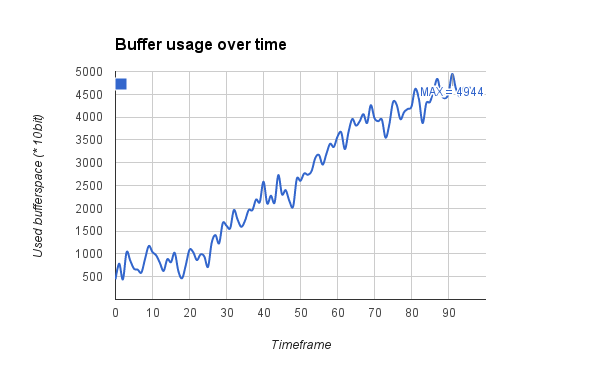
\includegraphics[width=1.0\textwidth]{images/mean-28.png}
		\caption{Using 28 percent mean occupancy.}
		\label{fig:28-occ}
\end{figure}

\paragraph{•}
As seen in \ref{fig:28-occ} the channel buffers fill up over time, and there is too much data for the serial outs to read.
For the first 15-20 time frames it seems somewhat stable, this is most likely because the simulation was "lucky" and picked low numbers of occupancies for the first part.
The buffer usage peaks at 4944 samples, but this number would continue to grow if the simulation was longer.
The difference when using a more realistic data model, instead of static occupancy becomes very clear in the resulting graph.
There is a lot more fluctuation in the buffer usage, and in comparison to the verification simulations, the resulting graph doesn't just increase in a linear fashion.
This is a good indication that both the behaviour of the simulation model and the normal distribution is working.


\subsubsection{2. 23\% Mean Occupancy}

\paragraph{•}
Since 28 percent mean occupancy was too much for the model to handle, the next simulation will try five percent less, i.e 23\%.
It uses the same setup in all other regards so that the results can be compared.
23 percent was chosen because it is far enough away from the first simulation to create a different result, without it being obvious whether the model will be able to handle it or not.

\begin{figure}[h!]
	\centering
		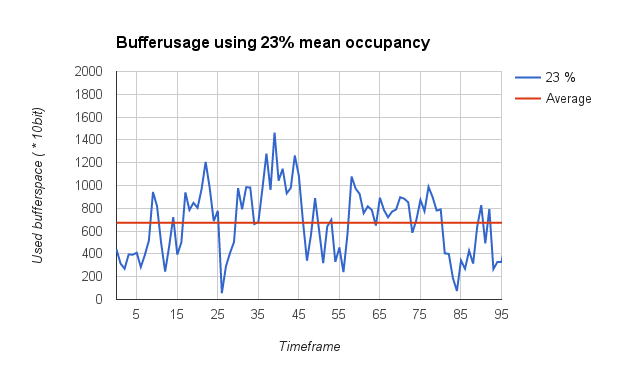
\includegraphics[width=0.9\textwidth]{images/23-occ.png}
		\caption{Results from simulation using 23\% mean occupancy.}
		\label{fig:23-occ}
\end{figure}

\paragraph{•}
The graph in \ref{fig:23-occ} shows shifting buffer usage, varying between 100 and 1500 samples.
However the graph shows that the model is able to read out the samples fast enough for the buffers not to overflow, always staying below the lowest of the suggested buffer sizes, 2k.
On average the buffers stored 675 samples at any time.
This is a number which is more than acceptable, and the simulation could most likely run forever and it would not matter.
To confirm this, a simulation using 10 000 time frames was run (\ref{fig:10k-23-occ}, and the results back up what the smaller one showed.
The results from it is compressed into a histogram over the occurrence of different buffer usage values.
It shows that most of the time the buffer usage is around 300-600, with an average of 473.
When running longer simulation it is only natural that it will shift more than the smaller ones, peaking at 2100 samples.
This means that a maximum buffer size of 2k is probably to small, as it is surpassed multiple times during 10 000 time frames.

\begin{figure}[h!]
	\centering
		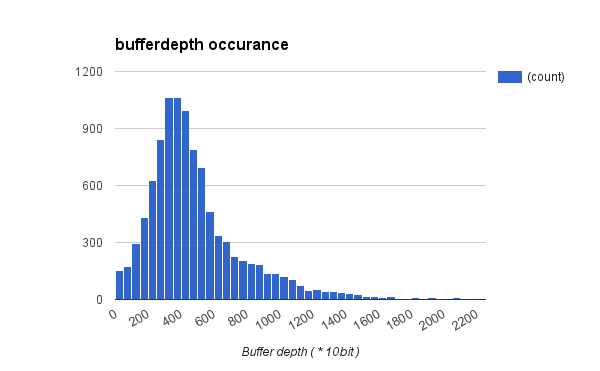
\includegraphics[width=0.9\textwidth]{images/10k-23-occ.png}
		\caption{Results from running 10 000 time frames using 23\% mean occupancy.}
		\label{fig:10k-23-occ}
\end{figure}

\paragraph{•}
The results gathered here show two very important things.
First of all it is clear that the model is able to level out the buffer usage when there is 23 percent occupancy, and it does so without any big spikes.
Second, it shows that when using 100 time frames the results gives an over estimate of the average usage.
When it ran for longer, it evened out to a smaller average, but with more and bigger spikes.
Now that it is clear that 23 percent is manageable, the next step is to find out where the limit it.
Given that 28 percent was to much, the limit is somewhere between 23 and 28 percent occupancy.

\subsubsection{3. Finding the limit} %Results unclear...

\paragraph{•}
Since finding the occupancy limit requires simulations using 24 to 27 percent occupancy, a combined graph, comparing the development of the buffer usage over time.
This will give a good overview of what happens both above and below the occupancy limit.

\begin{figure}[h!]
	\centering
		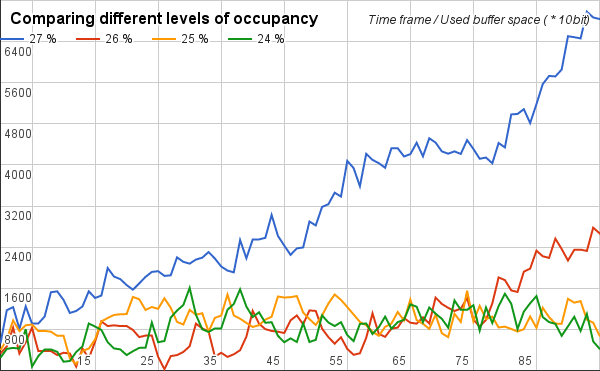
\includegraphics[width=1.0\textwidth]{images/24-27-occ.png}
		\caption{Results from using 24-27 percent occupancy.}
		\label{fig:24-27-occ}
\end{figure}

\paragraph{•}
The graph in \ref{fig:24-27-occ} shows results from all four different simulations.
The difference between 24 and 25 percent is not visibly seen, and it looks like they both are pretty stable over the course of 100 time frames.
However the difference in average buffer usage is still 150 samples, where 24 has around 850 and 25 has 1000.
1000 samples on average is starting to become high enough to cause issues with more time frames.
In this particular simulation it may be stable and without any large spikes, but this can be because that the simulation received occupancy levels which had a narrow distribution.
Another thing to note about the difference of 24 and 25 is that 24 has higher peaks then 25.
The reason for this can be seen when looking at their respective occupancy levels over time.
Even though the mean is one percent higher for 25, it has smaller range of values, and almost never gets multiple high occupancies in a row.
24 percent has on the other hand a wide distribution, with multiple values over the mean in a row. 

\begin{figure}[h!]
	\centering
		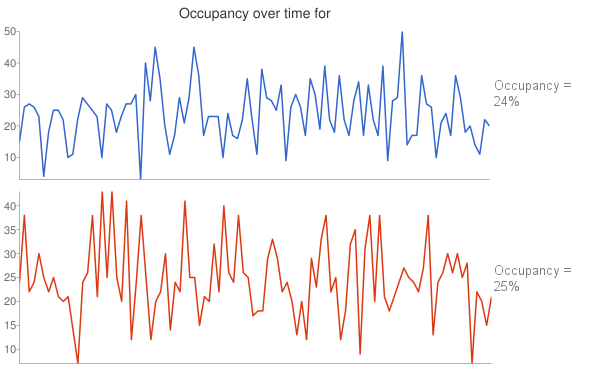
\includegraphics[width=1.0\textwidth]{images/occ-over-time.png}
		\caption{Showing occupancy over time using 24 and 25 percent.}
		\label{fig:occ-over-time}
\end{figure}

\paragraph{•}
When looking at 26 percent mean occupancy it can already be established that this is too much.
With a good distribution and lucky picking it can probably stay stable, but after a while the buffer usage will start to grow.
Not shockingly, this is definitely the case for 27 percent, increasing in buffer usage almost as fast as 28 percent.

\subsubsection{Evaluating the Results}

\paragraph{•}
From all simulations ran using the normal distribution, a graph showing the \gls{zs} compression factor for every level of occupancy has been compiled.
The compression factor is calculated by dividing maximum number of samples in a time frame with how many samples makes it though the \gls{zs}.
From prior calculations it is concluded that a compression factor of 2.5 is necessary in order for the serial outs to read fast enough.
If the compression factor of 2.5 is consistent with the occupancy limit found in the previous section, the results can be considered valid.

\begin{figure}[h!]
	\centering
		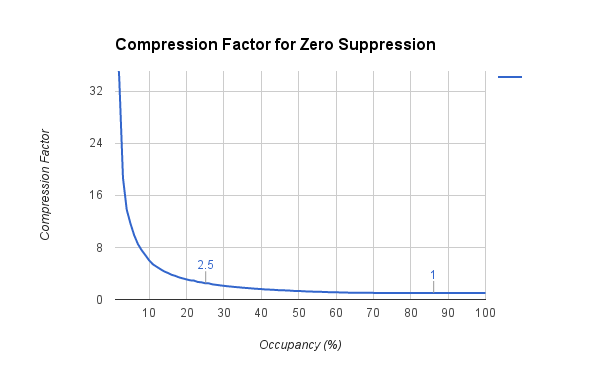
\includegraphics[width=1.0\textwidth]{images/comp-factor-results.png}
		\caption{The compression factor over level of occupancy.}
		\label{fig:comp-factor-results}
\end{figure}

\paragraph{•}
The compression factor graph shows that is reaches 2.5 at around 25 percent occupancy, decreasing faster and faster, giving an exponential function.
25 percent was exactly where the simulation model started to have trouble reading the data quickly enough, confirming that the results found were indeed valid.
A conclusion regarding this is that a 4k maximum buffer size should be enough with average occupancy lower then 25 percent.
This is only about three percent lower than the estimated average occupancy, and considering that the shape of the samples are as bad as possible for the \gls{zs} this is acceptable difference.


\subsection{Black Events}

\subsubsection{Preface}
\paragraph{•}
Using the black event dataset, the \gls{zs} and the Huffman encoding can be compared.
A crucial difference between the two different compression schemes is that the \gls{zs} is applied before the samples are stored in the buffers, while the Huffman encoding is applied while reading out from the buffers.
In other words, the \gls{zs} decreases the number of samples stored, while the Huffman effectively increases the readout speed by compressing each sample.
For the Huffman encoding there are two things that can happen.
Either it compresses the data enough that it manages to read the entire time frame before the next one is finished, which means that the buffer usage for every time frame will always be the size of an entire frame, i.e 1022 samples.
The other case is that the compression isn't good enough, and the buffers will overflow.
If the first case happens, then measuring the buffer usage seems pointless, therefore what is measured is the size of the time frame after compression.
This will be the closest way of comparing the results from both compression schemes.
Another thing that will be discussed is what difference black events with pileup will have in comparison to no pileup.


\subsubsection{1. Zero Suppression}

\paragraph{•}
The focus when looking at the \gls{zs} on the black events, will be the resulting buffer usage and not the compression factor itself.
The reasoning for this is that the \gls{zs} worst case has already been discussed.
The first results, which are displayed in \ref{fig:blackevents-zs} are using black events w/o pileup.
Results seems to show a rather low, and stable buffer usage, averaging out at about 330 samples, and peaking at 600 samples.
Since the data is collected from RUN 1, they have slightly less occupancy then what is expected for RUN 3, but it still has the most realistic shape available.

\begin{figure}[h!]
	\centering
		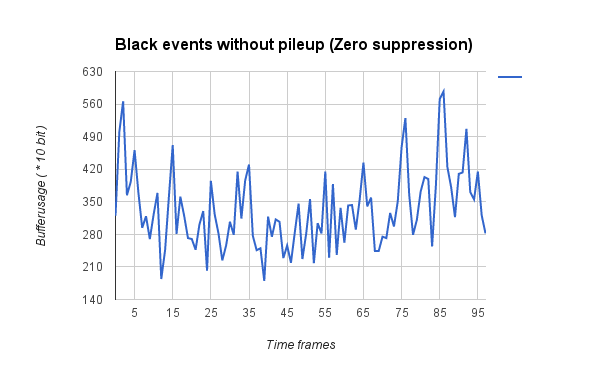
\includegraphics[width=1.0\textwidth]{images/blackevents-zs.png}
		\caption{Results from Black events w/o pileup using Zero suppression.}
		\label{fig:blackevents-zs}
\end{figure}

\paragraph{•}
One of the reasons for creating pileup data is to increase the amount of real samples, which possibly can give more interesting results than using plain black event data.
Running the simulation with the pileup data did indeed create interesting results, which can be seen in \ref{fig:blackevents-pileup-zs}.
As the previous results it stayed at around the same level during the entire simulation, but one can clearly see the increase in overall occupancy.
The pileup results peaked about 200 samples higher, and had an average of about 100 samples more.
Even though it is still manageable, it is clear that pileup has a real effect on the buffer usage when using \gls{zs}.

\begin{figure}[h!]
	\centering
		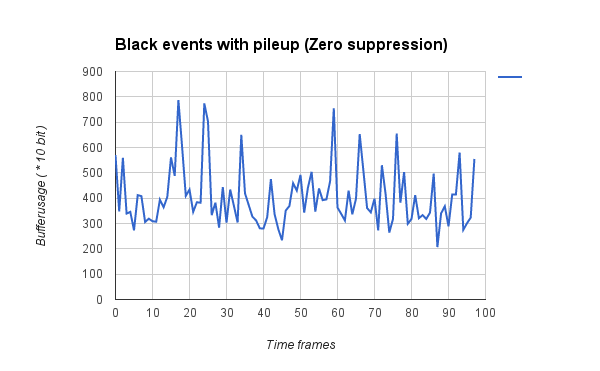
\includegraphics[width=1.0\textwidth]{images/blackevents-pileup-zs.png}
		\caption{Results from Black events with pileup using Zero suppression.}
		\label{fig:blackevents-pileup-zs}
\end{figure}

\subsubsection{2. Huffman Encoding}

\paragraph{•}
Now the same two simulations as before can be ran using the Huffman encoding instead of the \gls{zs}.
The expectation for the Huffman results is that the pileup should have less of an effect on the outcome, then when using \gls{zs}.
This is because that occupancy doesn't play as big of a role for Huffman, but instead the distribution of the sample values is what's important.

\begin{figure}[h!]
	\centering
		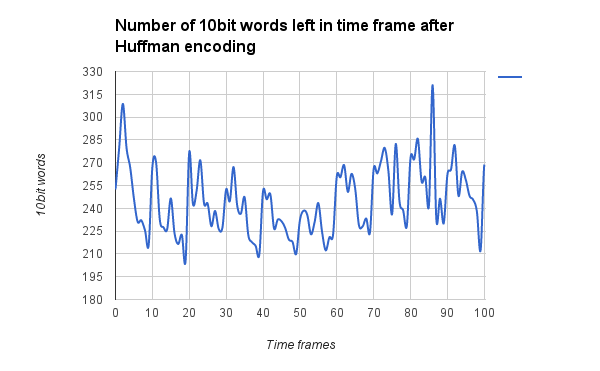
\includegraphics[width=0.9\textwidth]{images/blackevents-huffman.png}
		\caption{Results from Black events w/o pileup, using Huffman encoding.}
		\label{fig:blackevents-huffman}
\end{figure}

\paragraph{•}
The normal black event data was compressed enough for the serial outs to be able to read fast enough, therefore the buffer usage never surpassed the size of one full time frame.
In \ref{fig:blackevents-huffman} the compressed size of each time frame can be seen.
The graph shows that in most cases the Huffman encoding is able to compress the time frame to about 1/5 the original size, i.e a compression factor of four.
A full overview over the compression factors during the simulation is displayed as a histogram in \ref{fig:compression-factor-huffman}.
The factor goes down as low as 3.2, but on the other hand reaches as high as 4.95.
This isn't only more then the 2.5 that is needed, but also higher then what was expected of it.

\begin{figure}[h!]
	\centering
		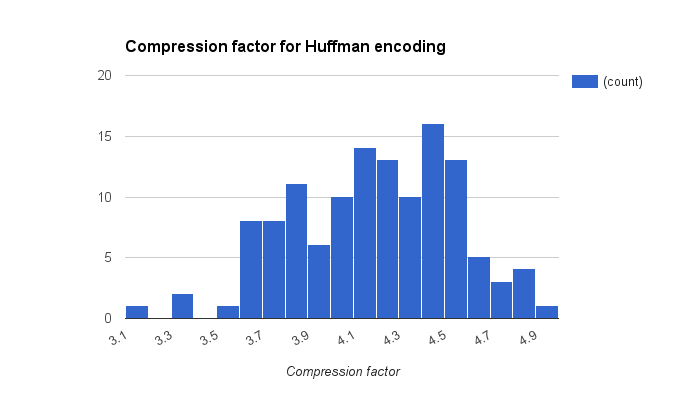
\includegraphics[width=1.0\textwidth]{images/compression-factor-huffman.png}
		\caption{Compression factor of Huffman on normal black events.}
		\label{fig:compression-factor-huffman}
\end{figure}

\paragraph{•}
Comparing the results from normal black events with the pileup results, there is a clear difference in regards to compression.
Reasons being that now that samples have been piled on top of each other, the difference between neighbouring time bins is bigger, which results in a worse Huffman table.
The compressed size of each time frame is now on average 100 words more than the normal black events, varying between 300 and 400 words.

\begin{figure}[h!]
	\centering
		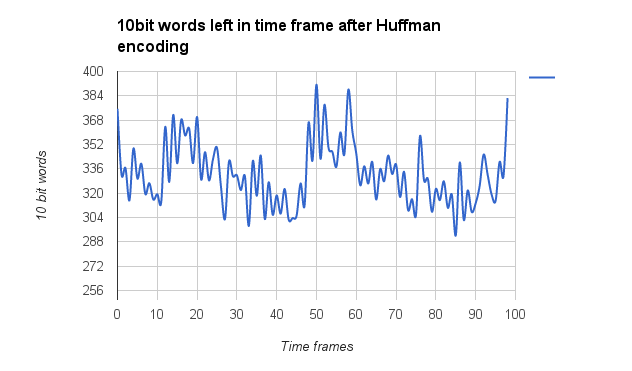
\includegraphics[width=1.0\textwidth]{images/blackevents-pileup-huffman.png}
		\caption{Compression factor of Huffman on piled up black events.}
		\label{fig:blackevents-huffman-pileup}
\end{figure}

\paragraph{•}
The pileup results show a definite decrease in the compression factor, as can be seen in \ref{fig:comp-huffman-pileup}.
However with an average compression factor of three the model is still able to read out data fast enough.
The factor varies between 2.6 and 3.5, always staying above the 2.5 limit, meaning that the model should never have any trouble.

\begin{figure}[h!]
	\centering
		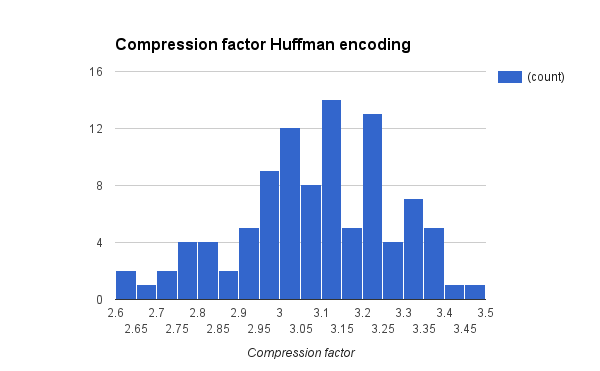
\includegraphics[width=1.0\textwidth]{images/compression-factor-pileup-huffman.png}
		\caption{Results from black events with pileup using Huffman encoding.}
		\label{fig:comp-huffman-pileup}
\end{figure}

\subsubsection{Evaluating the Results}

\paragraph{•}
Comparing the results when using \gls{zs} to using Huffman encoding ended up being harder then expected.
This is because of the difference in how they compress the data, one being applied before storing, and one after.
However there are multiple things to learn from these results.
For all the scenarios, the buffers never came close to being full.
It seems that for the black event dataset, the Huffman is able to perform better than \gls{zs}, but only by a small margin.
Huffman had a stronger decrease in performance than \gls{zs} when comparing normal black events, and pileup.
It can be argued that this is because the Huffman has a best case scenario, seeing as it uses the best possible Huffman table.
There is a significant difference between normal and pileup data, but not enough to be an issue.

\paragraph{•}
There was no way to see how the model behaved when Huffman didn't compress well enough, this is hopefully something that will be seen when trying the synthetic data made for RUN 3.


\subsection{Synthetic Data for RUN 3}

\subsubsection{Preface}
\paragraph{•}
Using the synthetic dataset made to simulate RUN 3 data, a final set of simulations can be performed.
As with the black events, the focus will be comparing \gls{zs} and Huffman encoding in terms of buffer usage, as well as look at the compression factor for the Huffman.
Hopefully there will be enough spread in the data to really test how the model behaves when the Huffman encoding isn't enough.
It is impossible to make any predictions here, as the properties of this dataset is unknown, and not previously been tested.

\subsubsection{1. Zero Suppression}

\paragraph{•}
For the \gls{zs} instead of taking the overall buffer usage now the channel with the highest average will be picked out and shown.
This gives a slightly different look into the model, focusing on the behaviour of a single channel.
Seeing as it is still the channel with the highest buffer usage it is still comparable to the overall highest shown in previous sections. 

\begin{figure}[h!]
	\centering
		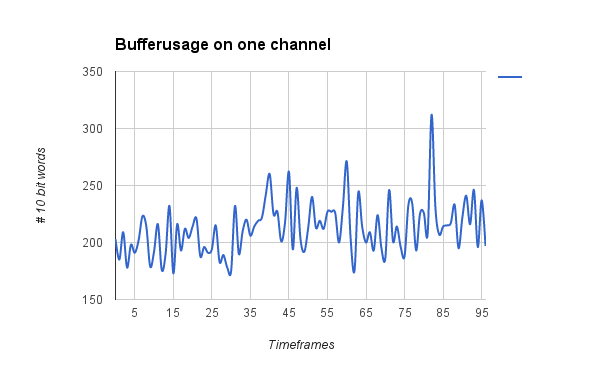
\includegraphics[width=1.0\textwidth]{images/bufferuse-one-channel-fake-pileup.png}
		\caption{Results from using \gls{zs} on synthetic data.}
		\label{fig:synthetic-zs}
\end{figure}

\paragraph{•}
Results show a unexpectedly low buffer usage, averaging out on about 220 samples.
In addition the difference from time frame to time frame is very low.
Comparing this to the results from the black events, it is significantly lower then those.
In \ref{fig:occ-synt-zs} the occupancy of the data is calculated.
The highest recorded occupancy found was 24 percent, with most being between 10 and 16 percent.
It seems that there isn't enough data to get any more decent results using \gls{zs}, but occupancy doesn't effect Huffman encoding in the same way.

\begin{figure}[h!]
	\centering
		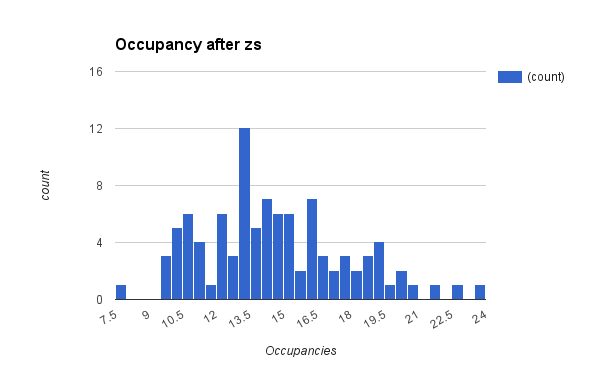
\includegraphics[width=1.0\textwidth]{images/occ-after-zs.png}
		\caption{Occupancy after \gls{zs}.}
		\label{fig:occ-synt-zs}
\end{figure}

\subsubsection{2. Huffman Encoding}

\paragraph{•}
Even though the results from using the \gls{zs} was disappointing, the dataset should give interesting results using Huffman encoding, which can be compared to the black event and pileup results.
As with those datasets, both the compressed size of the time frame, and the overall compression factor is what will be monitored, and presented.
In \ref{fig:synthetic-huffman} the graph shows that the average compressed size of a time frame is around 290 words.
What is strange, compared to the other datasets is the narrow difference in compressed size, with the largest time frame is 300, while the lowest is 285.


\begin{figure}[h!]
	\centering
		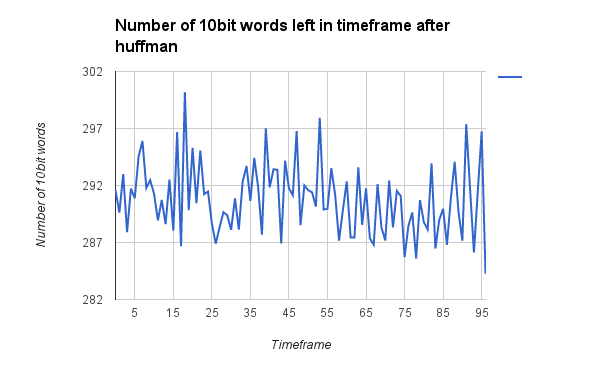
\includegraphics[width=1.0\textwidth]{images/huffman-fake-pileup.png}
		\caption{Results from using Huffman encoding on synthetic data.}
		\label{fig:synthetic-huffman}
\end{figure}

\paragraph{•}
The narrow difference in compressed size of a time frame seen in \ref{fig:synthetic-huffman} means that the dataset has very low, but even difference between consecutive time bins.
Since the Huffman encoding stores the difference between two time bins, the same difference has to be present a lot over all the time frames.
Looking at the histogram in \ref{fig:compression-factor-huffman-synt} displaying the compression factor, it shows that the difference in compression factor is very small.
It varies between 3.4 and 3.6, so to show the difference two decimals has to be used in the figure.

\begin{figure}[h!]
	\centering
		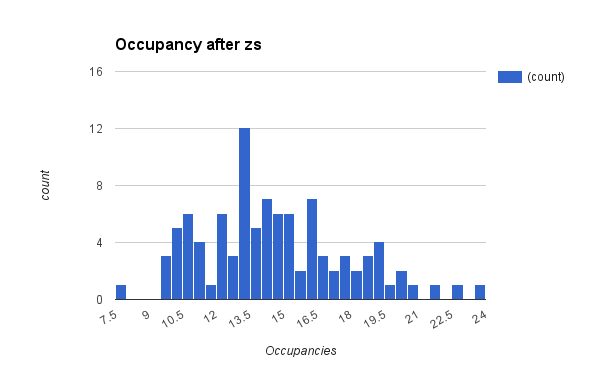
\includegraphics[width=1.0\textwidth]{images/huffman-comp-fake-pileup.png}
		\caption{Compression factor of using Huffman encoding on synthetic data.}
		\label{fig:compression-factor-huffman-synt}
\end{figure}

\subsubsection{Evaluating the Results}

\paragraph{•}
The results from using \gls{zs} was quite frankly uninteresting and there was not much to be learned from it, except that the dataset has a very low occupancy.
The Huffman results on the other hand was much more rewarding, and was comparable to the previous results found.
Comparing to the black events and pileup results, it lies somewhere in between them when it comes to compression.
Unlike previous results it has a very narrow result window, something not seen in the black event and pileup datasets.
One thing that all the Huffman results has in common is that it never reaches a compression factor of 5, meaning that between 2.6 and 4.9 is the best possible compression factor possible.
That being said, a factor over four will probably not be possible when using Huffman encoding in RUN 3.
Even though the hope for this simulation was to see how the model behaves when the Huffman encoding was not enough, the results was all in all educational.

\chapter{Conclusion and Future work}
\textit{Conclude the thesis, talk about the impact it has and its usefulness in future planing of the front end electronics.}

\paragraph{•}


\appendix
\chapter{Code Listings}
\label{cha:app-code}

\paragraph{•}
\begin{minipage}{\linewidth}
\lstinputlisting[caption=Channel header file.,firstline=1,lastline=24,label=lst:channel1]{codelistings/channel.cpp}
\end{minipage}

\paragraph{•}
\begin{minipage}{\linewidth}
\lstinputlisting[caption=Sampa header file.,firstline=1,lastline=26,label=lst:sampa2]{codelistings/sampa2.cpp}
\end{minipage}

\bibliography{biblio}{}
\bibliographystyle{unsrt}
\end{document}
